% !TeX spellcheck = es_ES
\documentclass[12pt, a4paper]{book} % Tipo de documento, tamaño de fuente y tamaño de página
\usepackage[T1]{fontenc} % Codificación de salida (tipos con tilde) y silabación castellana
\usepackage[utf8]{inputenc} % Reconocer tildes
\usepackage[english, spanish, es-tabla]{babel} % Idiomas para silabación y castellano principal; "tabla" en lugar de "cuadro"
\usepackage{graphicx} % Figuras PDF
\usepackage{setspace} % Interlineado
\usepackage{pdfpages} % Anexar PDF
\usepackage{xcolor} % Texto en color
\usepackage{breakcites} % Partir citas
\usepackage[font=onehalfspacing]{caption} % Anclas de figuras arriba e interlineado pie de foto 1,5
%\usepackage[showframe]{geometry} % Tamaño de página
\usepackage{arabicfront} % Números de página arábigos en frontmatter
\usepackage{etoolbox}
\usepackage{lscape}
\usepackage{enumitem} % Subapartados en itemize y enumerate
\usepackage{upquote}
\usepackage{dirtree} % Árboles de directorios sencillos
\usepackage{listingsutf8} % Meter código
\usepackage{accsupp} % Trabajar con el ActualText de listings
\usepackage{amsmath}
\usepackage[nottoc]{tocbibind} % Añadir bibliografía a índice
\usepackage{url}

%%%%%%%%%%%%% Itemize múltiple %%%%%%%%%%%%%%
\newlist{SubItemList}{itemize}{1}
\setlist[SubItemList]{label={$-$}}

\let\OldItem\item
\newcommand{\SubItemStart}[1]{%
	\let\item\SubItemEnd
	\begin{SubItemList}[resume]%
		\OldItem #1%
	}
	\newcommand{\SubItemMiddle}[1]{%
		\OldItem #1%
	}
	\newcommand{\SubItemEnd}[1]{%
	\end{SubItemList}%
	\let\item\OldItem
	\item #1%
}
\newcommand*{\SubItem}[1]{%
	\let\SubItem\SubItemMiddle%
	\SubItemStart{#1}%
}%
%%%%%%%%%%%%%%%%%%%%%%%%%%%%%%%%%%%%%%%%%%%%%

%%%%%%%%% Subsubsecciones numeradas %%%%%%%%%
\setcounter{tocdepth}{3}
\setcounter{secnumdepth}{3}
%%%%%%%%%%%%%%%%%%%%%%%%%%%%%%%%%%%%%%%%%%%%%

%%%%%%%%%%% Títulos reversibles %%%%%%%%%%%%%
\usepackage[explicit,
toctitles % Section marks en páginas impares
]{titlesec}

\titleformat{\chapter}[display]
{\normalfont\huge\bfseries\sloppy}
{\chaptertitlename\ \thechapter}{20pt}
{\hyperlink{toc}{\Huge#1}}

\titleformat{name=\chapter,numberless}
{\normalfont\huge\bfseries\sloppy}
{}{0pt}
{\hyperlink{toc}{\Huge#1}}

\titleformat{\section}
{\normalfont\Large\bfseries}
{\thesection.}{1em}{\hyperlink{toc}{#1}}

\titleformat{\subsection}
{\normalfont\large\bfseries}
{\thesubsection.}{1em}{\hyperlink{toc}{#1}}
%%%%%%%%%%%%%%%%%%%%%%%%%%%%%%%%%%%%%%%%%%%%%

%%%%%%%%% Encabezados reversibles %%%%%%%%%%%
\usepackage{fancyhdr}

% Comprueba si la expansión de 1 está vacía
\makeatletter
\newcommand{\ifemptymark}[1]{%
	\begingroup
	\sbox\z@{#1}%
	\expandafter\endgroup
	\ifdim\wd\z@=\z@
	\expandafter\@firstoftwo
	\else
	\expandafter\@secondoftwo
	\fi
}
\makeatother

\fancyhf{}
\fancyhead[LE]{\ifemptymark{\leftmark}{}{\hyperlink{toc}{\slshape\leftmark}}} % Quitar \leftmark en página después de \appendixpage
\fancyhead[RO]{\ifemptymark{\rightmark}{}{\hyperlink{toc}{\slshape\rightmark}}} % Solo si estamos dentro de una sección
\fancyfoot[LE,RO]{\thepage} % Headers
\renewcommand{\headrulewidth}{0pt} % Quitar línea inferior del header
\patchcmd{\chapter}{\thispagestyle{plain}}{\thispagestyle{fancy}}{}{} % Aplicar también a primera página de capítulo

\pagestyle{fancy}

% Quita "Capítulo 0" en encabezados del frontmatter
\makeatletter
\renewcommand\chaptermark[1]{%
	\markboth{\MakeUppercase{%
			\ifnum \c@secnumdepth >\m@ne
			\if@mainmatter
			\@chapapp\ \thechapter. \ %
			\fi
			\fi
			#1}}{}%
}
\renewcommand\@mkboth[2]{\markboth{#1}{}}
\makeatother
%%%%%%%%%%%%%%%%%%%%%%%%%%%%%%%%%%%%%%%%%%%%%

%%% Hiperenlaces y referencias reversibles%%%
% Poner el último para enlaces índice apuntando a página correcta
\usepackage[pagebackref, % Referencias reversibles
pdftex, % Preparar para PDF y partir hiperenlaces
pdfauthor={Carlos Clement Bellido},
pdftitle={Baco},
pdfsubject={Baco}]{hyperref}
\urlstyle{same} % Estilo URL normal

\renewcommand*{\backrefalt}[4]
{
	\ifcase #1
	\or        Citada en la página #2.
	\else      Citada en las páginas #2.
	\fi
}
\renewcommand*{\backrefsep}{, }
\renewcommand*{\backreftwosep}{ y }
\renewcommand*{\backreflastsep}{ y }

\usepackage[spanish,nameinlink]{cleveref} % autoref con minúscula inicial
\addto\captionsspanish{ % Cambiar nombre de secciones y subsecciones
	\crefname{section}{sección}{secciones}
	\crefname{subsection}{subsección}{subsecciones}
	\crefname{appendix}{anexo}{anexos}
}
\usepackage{crossreftools}
%%%%%%%%%%%%%%%%%%%%%%%%%%%%%%%%%%%%%%%%%%%%%

%%%%%%%%%%%%%%% Esquemas TikZ %%%%%%%%%%%%%%%
\usepackage{tikz}
\usepackage{varwidth} % Tablas en nodos TikZ
\usetikzlibrary{mindmap,shapes}
%%%%%%%%%%%%%%%%%%%%%%%%%%%%%%%%%%%%%%%%%%%%%

%%%%%%%%%%%%%%%%% Acrónimos %%%%%%%%%%%%%%%%%
\usepackage[acronym,toc,automake,ucmark=true,nogroupskip]{glossaries}
\makeglossaries
\newacronym{voip}{VoIP}{Del inglés, \selectlanguage{english}\textit{Voice Over Internet Protocol}\selectlanguage{spanish}, es un conjunto de recursos que permiten el envío de señales de audio por Internet empleando el protocolo IP}
\newacronym{linq}{LINQ}{Del inglés, \selectlanguage{english}\textit{Language Integrated Query}\selectlanguage{spanish}, permite, a los lenguajes .NET, capacidades de consulta de datos de forma nativa. Pertenece a la compañía Microsoft.}
\newacronym{fps}{FPS}{Del inglés, \selectlanguage{english}\textit{Frames Per Second}\selectlanguage{spanish}, indica la frecuencia de muestreo de imágenes por cada segundo.}
\newacronym{cli}{CLI}{Del inglés, \selectlanguage{english}\textit{command-line interface}\selectlanguage{spanish}, es una interfaz basada únicamente en líneas de texto simple.}
\newacronym{gui}{GUI}{Del inglés, \selectlanguage{english}\textit{graphical user interface}\selectlanguage{spanish}, es una interfaz basada imágenes y objetos gráficos para expresar información y acciones al usuario.}
%%%%%%%%%%%%%%%%%%%%%%%%%%%%%%%%%%%%%%%%%%%%%

%%%%%%%% Mensaje de página en blanco %%%%%%%%
\newcommand*{\blankpage}{%
	\vspace*{\fill}
	{\centering Está página ha sido dejada en blanco intencionadamente.\par}
	\vspace{\fill}}
\makeatletter
\renewcommand*{\cleardoublepage}{\clearpage\if@twoside \ifodd\c@page\else
	\blankpage
	\thispagestyle{fancy}
	\newpage
	\if@twocolumn\hbox{}\newpage\fi\fi\fi}
\makeatother
%%%%%%%%%%%%%%%%%%%%%%%%%%%%%%%%%%%%%%%%%%%%%

%%%%%%%%%%%%% Estilo del cover %%%%%%%%%%%%%%
\newcommand*{\coverpage}{%
	\vspace*{\fill}
	{\centering LALALALAAL.\par}
	\vspace{\fill}}
\makeatletter
%%%%%%%%%%%%%%%%%%%%%%%%%%%%%%%%%%%%%%%%%%%%%

%%%%%%% Lenguajes y cambio de captions %%%%%% 
\renewcommand*{\thelstnumber}{\protect\BeginAccSupp{ActualText={}}{\arabic{lstnumber}}\protect\EndAccSupp{}}
\AtBeginDocument{\renewcommand*{\theHlstnumber}{\arabic{lstnumber}}}
\makeatletter
\patchcmd{\lst@GLI@}% <command>
{\def\lst@firstline{#1\relax}}% <search>
{\def\lst@firstline{#1\relax}\def\lst@firstnumber{#1\relax}}% <replace>
{\typeout{listings firstnumber=firstline}}% <success>
{\typeout{listings firstnumber not set}}% <failure>
\makeatother
%\lstname\arabic{lstnumber}

% Java
\definecolor{pblue}{rgb}{0.13,0.13,1}
\definecolor{pgreen}{rgb}{0,0.5,0}
\definecolor{pred}{rgb}{0.9,0,0}
\definecolor{pgrey}{rgb}{0.46,0.45,0.48}

% XML
\definecolor{gray}{rgb}{0.4,0.4,0.4}
\definecolor{darkblue}{rgb}{0.0,0.0,0.6}
\definecolor{cyan}{rgb}{0.0,0.6,0.6}

% C#
\definecolor{bluekeywords}{rgb}{0.349,0.635,0.8}
\definecolor{lightgreenkeywords}{rgb}{0.356,0.752,0.631}
\definecolor{yellowgreenkeywords}{rgb}{0.756,0.5,0.670}
\definecolor{greencomments}{rgb}{0,0.5,0}
\definecolor{orangestrings}{rgb}{0.823,0.568,0.439}
\definecolor{types}{rgb}{0.17,0.57,0.68}
\definecolor{background}{rgb}{0.117,0.117,0.117}

% SQL
\definecolor{codegreen}{rgb}{0,0.6,0}
\definecolor{codegray}{rgb}{0.5,0.5,0.5}
\definecolor{codepurple}{HTML}{C42043}
\definecolor{backcolour}{HTML}{F2F2F2}
\definecolor{bookColor}{cmyk}{0,0,0,0.90}  
\color{bookColor}

\lstset
{
	tabsize=1,
	showspaces=false,
	showtabs=false,
	showstringspaces=false,
	breaklines=true,
	showstringspaces=false,
	prebreak=\mbox{\textcolor{red}{\BeginAccSupp{ActualText=$\rightarrow$}\space}},
	postbreak=\mbox{\textcolor{red}{\BeginAccSupp{ActualText=$\hookrightarrow$}\space}},
	inputencoding=utf8/latin1,
	breakatwhitespace=true,
	commentstyle=\color{greencomments},
	columns=fullflexible,
	basicstyle=\ttfamily\small,
	xleftmargin=\dimexpr-\leftmarginii-\leftmargini+60pt,
	extendedchars=true,
	escapeinside={(*@}{@*)},
	stringstyle=\color{orangestrings},
	numberstyle=\hypertarget{\lstname\arabic{lstnumber}}{\tiny\color{black}}
}

\lstdefinelanguage{Java}
{
	morecomment=[l]{//},
	morecomment=[s]{/*}{*/},
	morestring=[b]{"},
	emphstyle=[1]\color{pblue},
	emph=[1]
	{ 	
		public, class, import,
		package, extends, implements,
		new, null 
	}
}

\lstdefinelanguage{XML}
{
	morestring=[b]",
	morestring=[s]{>}{<},
	morecomment=[s]{<?}{?>},
	identifierstyle=\color{darkblue},
	keywordstyle=\color{cyan},
	morekeywords={xmlns,version,type}
}

\lstdefinelanguage{csh}
{
	rulecolor=\color{blue},
	rulesepcolor=\color{blue},
	morecomment=[l]{//},
	morecomment=[s]{/*}{*/},
	backgroundcolor=\color{backcolour},   
	commentstyle=\color{codegreen},
	emphstyle=[1]\color{darkblue},
	emph=[1]
	{ 	abstract, event, new, struct,
		as, explicit, null, switch,
		base, extern, object, this,
		bool, false, operator, throw,
		break, out, true,
		byte, fixed, override,
		case, float, params, typeof,
		private, uint,
		char, foreach, protected, ulong,
		checked, goto, public, unchecked,
		class, readonly, unsafe,
		const, implicit, ref, ushort,
		continue, in, return, using,
		decimal, int, sbyte, virtual,
		default, interface, sealed, volatile,
		delegate, internal, short, void,
		do, is, sizeof,
		double, lock, stackalloc,
		else, long, static, get,
		enum, namespace, string, set,
		async, await, var},
	emph=[2]
	{	StreamReader, Dictionary, DateTime, Environment,
		Program, Console, Queue, Stack,
		List, StreamWriter, KeyValuePair, Directory,
		File, Rally, Equipo, Interruptor,
		Bombilla, Task, Random, Stopwatch,
		Image, Timer, Texture2D, BitmapData,
		MemoryStream, Action, VideoFrame, FrameMapping,
		Client, ServerObject, SharpDXException, ResultCode,
		Debug, Thread, GC, Exception
	},
	emphstyle=[2]\color{lightgreenkeywords},
	emph=[3]
	{	ConsoleKey, OutputDuplicateFrameInformation, DataBox, Rectangle,
		MapMode, PixelFormat, Bitmap, ImageLockMode,
		IntPtr, Point, ServerFlag, SenderObject,
		SenderFlags
	},
	emphstyle=[3]\color{yellowgreenkeywords},
	emph=[4]
	{	while, if, for, catch, 
		try, finally
	},
	emphstyle=[4]\color{codepurple},
	breaklines=true,                 
	captionpos=b,                                
	numbers=left,                                 
	showspaces=false,                
	showstringspaces=false
}

\lstdefinelanguage{sql}{
	backgroundcolor=\color{backcolour},   
	commentstyle=\color{codegreen},
	emphstyle=[1]\color{bluekeywords},
	emph=[1]
	{
		 CREATE, TABLE, INSERT, INTO,
		 DATABASE, USE, INT, IDENTITY,
		 PRIMARY, KEY, VARCHAR, BIT,
		 DEFAULT, FOREIGN, REFERENCES,
		 VALUES
	},
	morestring=*[d]{'},
	stringstyle=\color{codepurple},
	basicstyle=\footnotesize,
	breakatwhitespace=false,         
	breaklines=true,                 
	captionpos=b,                                
	numbers=left,                                 
	showspaces=false,                
	showstringspaces=false  
}
\renewcommand{\lstlistingname}{C\'{o}digo} % Listing -> Código
\renewcommand{\lstlistlistingname}{Lista de \lstlistingname s}% List of Listings -> Lista de Códigos 
%%%%%%%%%%%%%%%%%%%%%%%%%%%%%%%%%%%%%%%%%%%%%

\title{Baco: \selectlanguage{english}\textit{streaming}\selectlanguage{spanish} de vídeo y VoIP sobre TCP}
\author{Carlos Clement Bellido\\\href{mailto:carlos.clement@iesdoctorbalmis.com}{carlos.clement@iesdoctorbalmis.com}}
\date{Alicante, \today}

\begin{document}
	
	\onehalfspacing % Interlineado 1,5
	\setlength{\parskip}{\baselineskip/3} % Espacio entre párrafos 2
	\setlength{\parindent}{0pt} % No identar primera línea de párrafo
	
	\frontmatter
	\maketitle
	\cleardoublepage % Hypertarget en posición correcta
	\hypertarget{toc}{} % Hypertarget sobre título de índice 
	\tableofcontents
	\printglossary[type=\acronymtype,nonumberlist,title={Acrónimos}]
	\mainmatter
	
	\chapter{Introducción}
	Baco es una aplicación de escritorio orientada a sistemas Windows y enfocada a la comunicación entre usuarios en Internet.\\
	El repositorio se encuentra en \href{https://github.com/CarlosClementBellido/Baco}{GitHub} (\href{git-client://clone?repo=https\%3A\%2F\%2Fgithub.com\%2FCarlosClementBellido\%2FBaco}{clonar proyecto}) bajo licencia \selectlanguage{english}\textit{GNU General Public License v3.0}\selectlanguage{spanish}.
		\section{Objetivo} \label{sc:objetivo}
		Se busca como objetivo suplir las carencias que las actuales \acrshort{voip} poseen: un control más técnico sobre la comunicación con los usuarios, facilidades para las tareas ordinarias, optimización de flujo de datos... todo ello acompañado de una mentalidad de software libre: los fuentes del programa están a disposición de los usuarios para que puedan compilar y usar su propia copia del programa. La idea es que cada usuario pueda aportar sus modificaciones a la aplicación oficial y, los trabajadores de Baco contemplen si dicha modificación propuesta pueda ser incluida en la aplicación oficial (en forma de nueva versión). 
		\section{Justificación}
		Debido a que las principales aplicaciones de comunicación por Internet no daban la posibilidad de manejar los aspectos complejos de las comunicaciones se ha desarrollado esta aplicación. Dichos controles sobre el flujo de datos sobre Internet se entrará en detalle más adelante.\\
		Debido a que, actualmente, predomina el software privativo, se ha optado por liberar el código para que la comunidad haga de él lo que le plazca.
		\section{Análisis de lo existente}
		En el mercado, existen multitud de aplicaciones VoIP, pero ninguna de ellas da las opciones que Baco proporciona. Si se continúa el desarrollo puede llegar a ser una competencia feroz ante los principales competidores: Discord, Skype, TeamSpeak... una de las características que no poseen estos competidores es la opción de suscripción a canales RSS. La pantalla principal de Baco nos muestra los canales RSS a los que el usuario está suscrito e implementa un visor de HTML cuyo motor de renderizado es Gecko e incorpora bibliotecas de Mozilla Firefox.\\
		Baco no solo posee un visor de RSS, también nos proporciona un sistema de llamadas por Internet. Estas llamadas son entre amigos y pueden ser de cuantas personas se quiera. Además se da la opción de compartir en tiempo real la pantalla manejando parámetros de envío: tasa de capturas por segundo (\acrshort{fps}) y calidad de captura (menor calidad aumenta la velocidad de transmisión y reduce el peso de la imagen).\\
		Mientras se está en llamada no se transmite continuamente la voz del usuario: solamente se envía en el caso de pasar un umbral mínimo y no rebasar un umbral máximo. Estos umbrales pueden modificarse en las opciones de Baco, dentro de las cuales podremos encontrar más campos a modificar en el apartado de audio (todas las opciones modificables se encuentran con un botón de restablecimiento al valor por defecto).\\
		Por otra parte, dejando de lado la aplicación de cliente, tenemos un servidor que es el encargado de gestionar el funcionamiento de la aplicación. El servidor es una aplicación de consola y su función es controlar todo cuanto sucede en los clientes y en el propio servidor. Mientras el cliente esté dentro de la aplicación estará conectado al servidor.\\
		Debido a que es \acrshort{cli} se ha implementado un sistema básico de comandos para el manejo y control en tiempo real del servidor.\\
		La API es otra CLI con la diferencia que acepta peticiones HTTP y envía datos por red, es decir, actúa a modo de servidor. Ello es capaz de hacerlo gracias a \hyperlink{entity}{Microsoft.EntityFrameworkCore}.\\
		Las peticiones HTML se resuelven y se retorna el JSON especificado. Los datos del JSON salen del proyecto Service, el cual es una biblioteca de clases que se encarga de la conexión con la base de datos mediante un contexto. Se hablará de ello mas adelante, en la \crthypercref{sbc:db}. Service hace las consultas al contexto de la base de datos con \acrshort{linq}.
				
	\chapter{Necesidades empresariales para el desarrollo}
	Dado que Baco es un programa de código abierto, los ingresos vienen por parte de las empresas que quieran utilizar este software. Los usuarios particulares podrán obtener una copia del programa de forma gratuita mientras que las empresas deberán pagar para obtenerlo. Puesto que la empresa tiene que pagar por el software se le ofrecen funcionalidades especiales:
	\begin{itemize}
		\item Soporte a los posibles problemas o errores que tengan con la aplicación
		\item Certificado de comunicaciones entre usuarios
		\item Cifrado de datos
		\item Posibilidad de un servidor privado
	\end{itemize}
		\section{Recursos humanos}
		Al ser una empresa de software y con el panorama en la actualidad (la crisis de la COVID-19) se ha demostrado que el trabajo desde las casas de los trabajadores no es sino una ventaja para la misma empresa. Es por ello que Baco opta por una empresa descentralizada, sin ningún sitio fijo de trabajo. Con esto abaratamos los costes que suponga la compra o el alquiler del sitio de trabajo. En caso de reunión se dispondrá de un lugar para ello (comprado o alquilado por la empresa). No obstante se facilitarán los medios y materiales necesarios para los trabajadores. Entiéndase uno de los medios principales la comunicación entre los compañeros; para lograr esta comunicación se usará Baco, de este modo los mismos programadores estarían probando el programa todo el tiempo.
			\subsection{Trabajadores}
			Debido a que Baco no es gratuito con fines empresariales habremos de tener una sección de comerciales que se encarguen de la contratación del software por parte de las empresas y otra de marketing para darse a conocer a ellas. Y por último tendríamos la parte imprescindible de la empresa, los programadores.\\
			El salario de los trabajadores se ajustará a los establecido por el convenio del sector.
			\subsection{Contratos}
			Debido a que se va a utilizar la línea de Internet por parte de los trabajadores desde su domicilio se pagará una cantidad determinada al trabajador en nómina en concepto de gastos por uso de Internet, telefónicos y electricidad.\\
			Todos los trabajadores tendrán un sistema de cobro complementario al salario por objetivos a modo de incentivo, así como un contrato a tiempo completo ordinario.\\
			Los tipos de trabajadores podrían estructurarse de las siguiente forma:
			\begin{itemize}
				\item Programadores: la empresa proveerá los programas necesarios a los trabajadores para la realización de los trabajos. En esta categoría los programadores se enfrentarían a: desarrollo de nuevas funcionalidades de Baco, implementación de funcionalidades cedidas por la comunidad (como bien se explicó en la \crthypercref{sc:objetivo}) y mantenimiento de la página web, la cuál será el medio de descarga tanto como para empresas como para particulares.
				\item Comerciales: en el supuesto de visitas presenciales se pagará un plus de vestuario y transporte, ademas de los medios necesarios para el desplazamiento al cliente (si es requerido, la empresa alquilará a una empresa un vehículo para el empleado). La función de los comerciales será visitar empresas con el fin de lograr contratos con ellas para la cesión de software.
				\item Publicistas: estos serán los encargados de la parte que el publico verá de Baco. La publicidad estará enfocada en empresas y particulares, centrándose principalmente en la publicidad en Internet. Al igual que los programadores, se les proporcionará acceso a cualquier tipo de software que requieran.
				\item Relaciones públicas (RR.PP.): será la primera persona con quien los particulares y las empresas hablarán si quieren contactar con Baco. Será quien redirija a los comerciales las empresas que se hayan interesado por el software, reenvíe las ideas que haya tenido la comunidad para implementar a Baco a los programadores, lleve las redes sociales e informe a los publicistas del impacto que haya tenido la publicidad de la empresa en el público.
			\end{itemize}
			El hecho de que haya varias categorías no implica que una persona no pueda realizar más de una, por ejemplo, un publicista puede también encargarse de la parte de RR.PP., o un comercial puede ser publicista. Si esto se diera supondría un incremento en el salario del trabajador. Este incremento junto con el complemento por trabajo realizado supone flexibilizar las capacidades de los trabajadores y no centrarlos solo en una materia dentro de la empresa, ya que esto podría suponer a la larga un decremento del interés. La empresa buscará por encima de todo unos trabajadores felices aunque ello suponga una pérdida de capital.
			\subsection{Seguridad Social}
			Las obligaciones en materia de seguridad social se dan a la hora de su puesta en marcha. Podemos dividirla en dos apartados:
			\begin{itemize}
				\item Trámites generales:
				\begin{itemize}
					\item Alta de los socios y administradores en los regímenes de la Seguridad Social: debido a que la empresa está creada por una única persona y puesto que, evidentemente, se posee más del 50\% del capital el régimen será el de autónomos.
				\end{itemize}
				\item Trámites en caso de contratar trabajadores:
				\begin{itemize}
					\item Inscripción de la empresa: cuando, por vez primera, se quiera contratar trabajadores se habrá de solicitar la inscripción como empresario en la Tesorería General de la Seguridad Social (TGSS).
					\item Afiliación de trabajadores (en el supuesto de que no estén afiliados): aquellos trabajadores que vayan a ser contratados y no tengan número de filiación (NAF) habrán de solicitarlo. Debe solicitarse a instancia del empresario.
					\item Alta de los trabajadores en el Régimen de la Seguridad Social: cada trabajador habrá comunicarse su alta en el Régimen de la Seguridad Social correspondiente.
				\end{itemize}
			\end{itemize}
			
		\section{Prevención de riesgos laborales}
		Dado que es una empresa de software no posee demasiados riesgos laborales graves. Los principales riesgos son obvios, la salud visual de los trabajadores, así como la física que se de a causa de malos hábitos por parte del trabajador. También cabe mencionar que los comerciales, al tener la opción del desplazamiento con vehículo tengan que ser tenidos en cuenta por posibles percances durante los trayectos a las empresas.
			\subsection{Riesgos laborales y medidas preventivas}
			A continuación se enumerarán los principales riesgos laborales junto con los motivos del riesgo y las medidas preventivas correspondientes:
			\begin{itemize}
				\item Contactos eléctricos: puesto que los trabajadores trabajan con instrumentos conectados a la corriente queda constancia de que pueda suponer un riesgo a considerar.
				\begin{itemize}
					\item No manipular ni intentar reparar equipos de trabajo conectados a la electricidad.
					\item No desconectar aparatos tirando directamente del cable de corriente.
					\item No usa regletas (comúnmente conocidas como <<ladrones>>) que no garanticen la continuidad del conductor a tierra ni las conecte en serie.
					\item Asegurarse de que  los cables no se encuentran aplastados o dañados.
					\item Desconectar los equipos cuando no se usen.
					\item Evitar limpiar con líquidos cualquier equipo conectado a la red eléctrica.
					\item No manipular instalaciones eléctricas con las manos húmedas.
				\end{itemize}
				\item Condiciones ambientales generales: exposición a iluminación inadecuadas que puedan dar lugar a problemas visuales.
				\begin{itemize}
					\item Adecuar la iluminación a las exigencias visuales.
					\item Iluminar correctamente las zonas oscuras.
					\item Para evitar reflejos o fuertes contrastes ninguna ventana se encontrará ni detrás ni delante de una pantalla.
					\item Las ventanas han de tener elementos que amortigüen la entrada de luz para que, en el caso de molestias, pueda regularse la luz.
					\item La iluminación artificial habría de ser difusa y proveniente de fuentes de luz de gran superficie.
					\item Reparar de manera inmediata aquellas fuentes de luz que pudieran parpadear.
					\item Para la prevención de la sequedad de ojos y mucosas se recomienda una elevada humedad relativa y la ventilación diaria del área de trabajo.
					\item La temperatura habría de estar a un nivel con el que el trabajador esté a gusto.
					\item Aislamiento de fuentes de ruido para evitar la exposición prolongada a ruidos elevados.
				\end{itemize}
				\item Condiciones del puesto de trabajo: a consecuencia del entorno, organización, diseño del puesto de trabajo, carga mental, factores psicosociales y desempeño pueden producirse daños para la salud. Es por ello que habrán de ser analizados antes de que se produzcan.
				\begin{itemize}
					\item Una correcta posición a la hora de sentarse:
					\begin{itemize}
						\item Espalda apoyada en el respaldo y en ángulo recto con respecto a las piernas.
						\item La altura de la silla ha de ser aquella sobre la cual los codos puedan descansar sobre la mesa formando un ángulo de 90º.
						\item Si los pies no llegan al suelo se requerirá de un reposapiés.
					\end{itemize}
					\item Distribuir los elementos de trabajo de forma que estén más cerca los que más utilizados.
					\item El espacio permitirá cambios de postura y movimientos.
					\item Al realizarse en el domicilio el trabajo deberá estar aislado/separado para que permita cierta intimidad.
					\item Planificación de las actividades a realizar y los descansos a realizar. 
					\item Evitar trabajar más de cuatro horas seguidas y cada dos realizar una pausa para relajar las musculatura.
				\end{itemize}
				\item Sobre esfuerzos: dado que el manejo del teclado y el ratón es imprescindible para la realización del trabajo, ello se considera como posible causa de lesiones como el síndrome del túnel carpiano (causado por el uso continuado del ratón).
				\begin{itemize}
					\item Evitar apoyar el teléfono a la hora de hablar entre en hombro y la cabeza.
					\item Los giros sobre la silla habrían de hacerse haciendo uso de los pies y no de giros bruscos de tronco.
					\item No forzar la postura para alcanzar objectos que se encuentren lejos: levantarse para alcanzarlos.
					\item No permanecer estático durante un tiempo excesivo.
					\item Sentado no se habrían de manipular cargas.
				\end{itemize}
				\item Usuarios de P.V.D. (Pantalla de Visualización de Datos): la empresa deberá de analizar la posibilidad de la aparición en sus empleados de daños relacionados con el manejo continuo de pantallas alfanuméricas o gráficas (recogido en el \href{https://www.boe.es/buscar/doc.php?id=BOE-A-1997-8671}{Real Decreto 488/1997} del 14 de Abril).
				\begin{itemize}
					\item Colocar la pantalla lo más centrada para evitar molestias posturales del tronco y cervicales.
					\item La pantalla deberá de estar más baja que el nivel de los ojos y de 60 a 80 cm. Nunca habrá de estar a menos de 40 cm o superior a 90 cm.
					\item Parpadear frecuentemente para evitar la sequedad ocular y realizar pausas periódicas.
					\item Desviar la vista periódicamente a objetos a media y larga distancia.
					\item Mantener los antebrazos apoyados en la silla o en la mesa para evitar la suspensión de las muñecas en el uso del teclado y el ratón.
				\end{itemize}
			\end{itemize}
		\section{Iniciativa emprendedora}
		Para la creación de la empresa se deben de especificar ciertos detalles de ella, como la forma jurídica, cuál será el proceso de constitución y trámites para la puesta en marcha.
			\subsection{Forma jurídica}
			Debido a que las trabajadores realizarían su trabajo desde casa y la dirección de la empresa residiría en una oficina cuyo coste mensual no sería elevado se ha elegido la forma jurídica de Sociedad de Responsabilidad Limitada. El teletrabajo está regulado por el Acuerdo Marco Europeo sobre Teletrabajo \cite{Teletrabajo_en_Espana_acuerdo_marco_y_administracion_publica}, \cite{Telefonica_Espana}.
			\subsection{Tramites administrativos}
			Consideraremos trámites administrativos únicamente los de constitución y puesta en marcha de la sociedad.
				\subsubsection{Constitución}
				\begin{itemize}
					\item Registro Mercantil Central: Certificación negativa del nombre de la sociedad
					\item Agencia Tributaria (AEAT): Número de identificación fiscal
					\item Notario: Escritura pública (la cual deberá presentarse a inscripción en el Registro Mercantil Provincial)
					\item Consejerías de Hacienda de las CC.AA: Impuesto sobre transmisiones patrimoniales y actos jurídicos documentados
					\item Registro Mercantil Provincial: Inscripción de la empresa en el Registro  
				\end{itemize}
				\subsubsection{Puesta en marcha}
				\begin{itemize}
					\item AEAT:
					\begin{itemize}
						\item Alta en el Censo de empresarios, profesionales y retenedores
						\item Impuesto sobre Actividades Económicas (exentas las empresas de nueva creación durante los dos primeros ejercicios)
					\end{itemize}
					\item TGSS:
					\begin{itemize}
						\item Alta de los socios y administradores en los regímenes de la Seguridad Social
						\item Inscripción de la empresa
						\item Afiliación de trabajadores (en el supuesto de que no estén afiliados)
						\item Alta de los trabajadores en el Régimen de la Seguridad Social
					\end{itemize}
					\item Registro Mercantil Provincial:
					\begin{itemize}
						\item Legalización del Libro de actas, del Libro registro de socios, del Libro-registro de acciones nominativas y del Libro registro de contratos entre el socio único y la sociedad
						\item Legalización del Libro Diario y del Libro de Inventarios y Cuentas Anuales
					\end{itemize}
					\item Autoridades de certificación: Obtención de un certificado electrónico
					\item Ayuntamientos: Licencia de actividad
					\item Otros organismos oficiales y/o registros: Inscripción en otros organismos oficiales y/o registros
					\item Servicio Público de Empleo Estatal: Alta de los contratos de trabajo
					\item Consejería de Trabajo de la CCAA: Comunicación de apertura del centro de trabajo
					\item Inspección Provincial de Trabajo: Obtención del calendario laboral
					\item Oficina Española de Patentes y Marcas: Registro de signos distintivos (opcional)
				\end{itemize}
	\chapter{Requisitos funcionales de la aplicación}
	Como bien se ha comentado en la \crthypercref{sc:objetivo}, Baco ofrece manejar a niveles técnicos distintos aspectos, como la tasa de bits, el número de canales de audio, el búfer de sonido, la tasa de fotogramas que se envía, la calidad con la que se transmite vídeo... debido a esto, Baco sería ideal para aquellas personas que quieran modificar aspectos técnicos dentro de la aplicación (mediante las opciones que esta da), y las que quieran modificar los fuentes del programa para realizar acciones específicas (\selectlanguage{english}\textit{open source}\selectlanguage{spanish}). También, debido a su simplicidad, puede ser usado por personas sin conocimientos informáticos relacionados con los tocados por la aplicación.\\
	En general: Baco es una alternativa sencilla, simple y enfocada a todos los públicos.
	
	\chapter{Análisis y Diseño}
	Para que la comunicación entre los usuarios sea posible ha de hacerse mediante un servidor pasarela. Dicho servidor es el encargado de registrar los usuarios conectados, mandar y almacenar mensajes de texto entre usuarios (almacenar aquellos que no puedan llegar al usuario destino), establecer llamadas entre usuarios (envío de audio y vídeo) y acceder al API REST. Los clientes acceden a la base de datos por medio del servidor, de este modo únicamente han de hacer una conexión por Internet; si el cliente está conectado al servidor, está en contacto con todos sus amigos y con la base de datos.
		\section{Diagrama de la arquitectura}
		La arquitectura de Baco es relativamente sencilla: un usuario tiene amigos y puede comunicarse con ellos. Las comunicaciones se establecen mediante el servidor de Baco, quien se encarga de establecer las comunicaciones entre los usuarios.\\
		Supongamos que un usuario (A) quiere enviar un mensaje de texto a un amigo (B) que está conectado:\\\\
		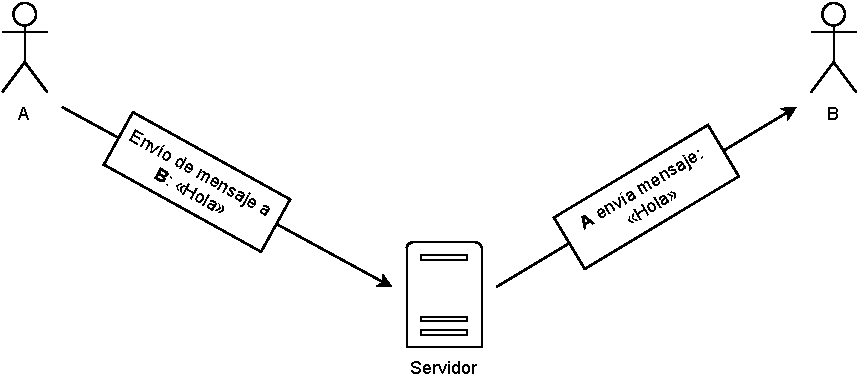
\includegraphics[width=\textwidth,height=\textheight, keepaspectratio]{img/BasicTextCommDiagram.pdf}
		El funcionamiento es simple. En el supuesto de que B no esté conectado, cuando lo esté el mensaje le llegaría de igual manera.\\\\
		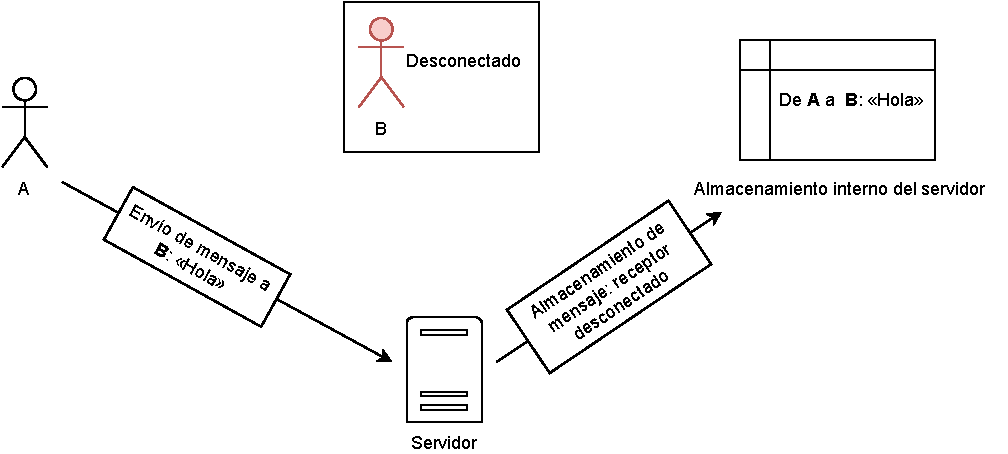
\includegraphics[width=\textwidth,height=\textheight, keepaspectratio]{img/BasicTextCommNotConnDiagram.pdf}\\
		Usuario B se conecta:\\\\
		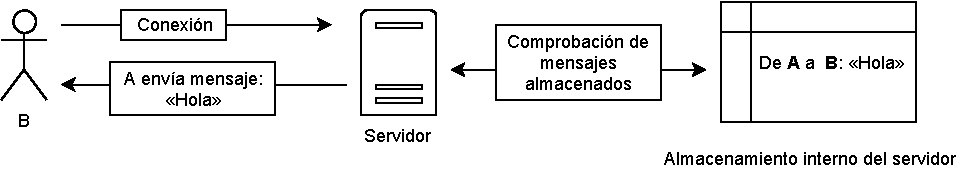
\includegraphics[width=\textwidth,height=\textheight, keepaspectratio]{img/BasicTextCommStoredDiagram.pdf}\\
		\newpage
		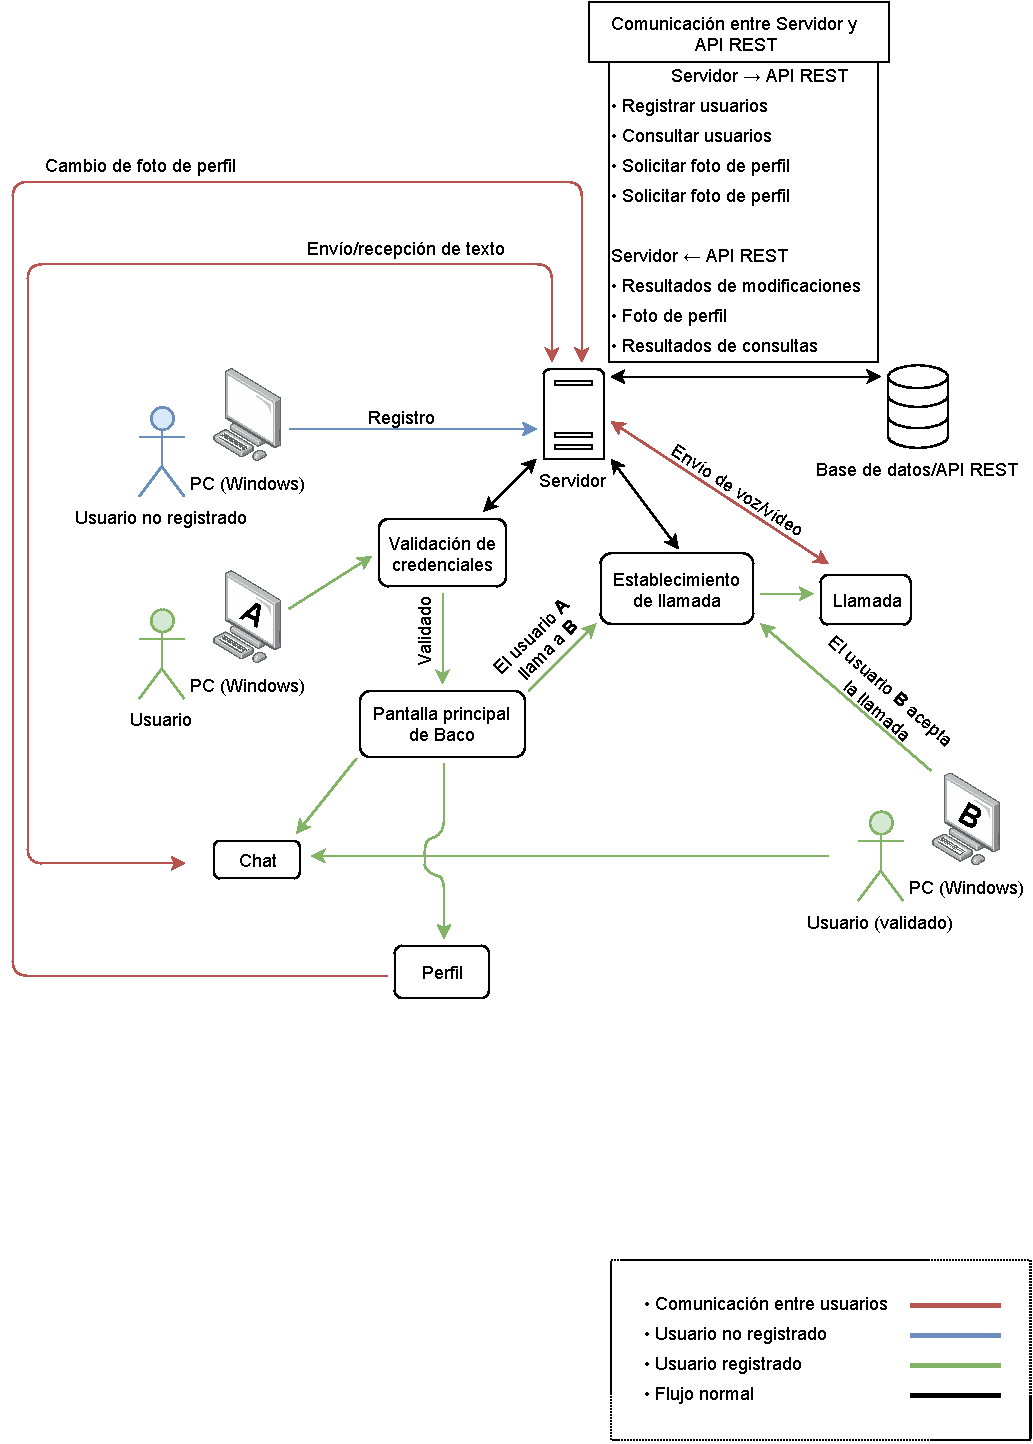
\includegraphics[width=\textwidth,height=\textheight, keepaspectratio]{img/ArchitectureDiagram.pdf}\\
		Baco no solo es capaz de enviar a un único destinatario, es capaz de manejar grupos, es decir, un usuario envía un mensaje a múltiples usuarios y estos lo reciben en la misma conversación.\\
		Si sustituimos los mensajes de texto por vídeo y audio obtenemos el sistema de llamada de Baco. Esto implica que las comunicaciones VoIP no han de ser exclusivamente de dos personas, sino que pueden ser de cuantas se quiera.
		\section{Diagrama de casos de uso}
		A continuación se muestra el diagrama simplificado de casos de uso. En él podremos apreciar las diversas acciones que puede realizar el cliente (una vez registrado):
		\begin{itemize}
			\item Llamar a amigos
			\item Mandar y recibir mensajes de texto
			\item Ver y actualizar la imagen de perfil
			\item Ver los canales RSS que el usuario está suscrito y suscribirse a más
			\item Modificar opciones de audio
		\end{itemize}		
		\newpage
		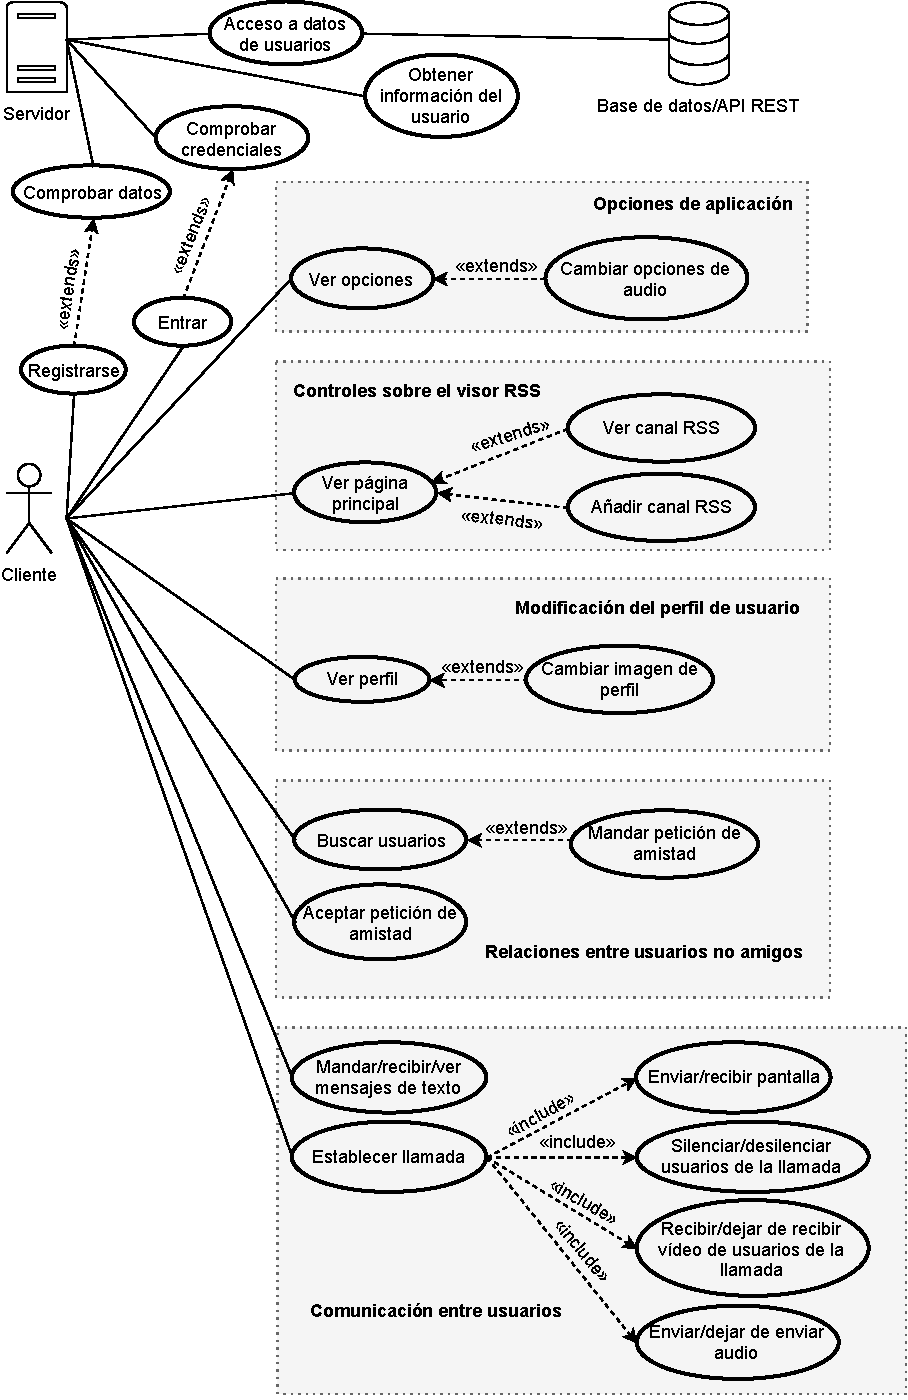
\includegraphics[width=\textwidth,height=\textheight, keepaspectratio]{img/UseCaseClient.pdf}\\
%		\newpage
		\section{Diagrama de clases}
		Debido a la complejidad de las clases en la solución de proyectos, se van a simplificar las relaciones. Se mostrarán los diagramas de clases del cliente y del servidor dado que el proyecto que maneja la API no posee complejidad alguna en este aspecto.
			\subsection{Cliente}
			Las páginas siguientes mostrarán el diagrama de clases de Baco (aplicación de cliente).\\
			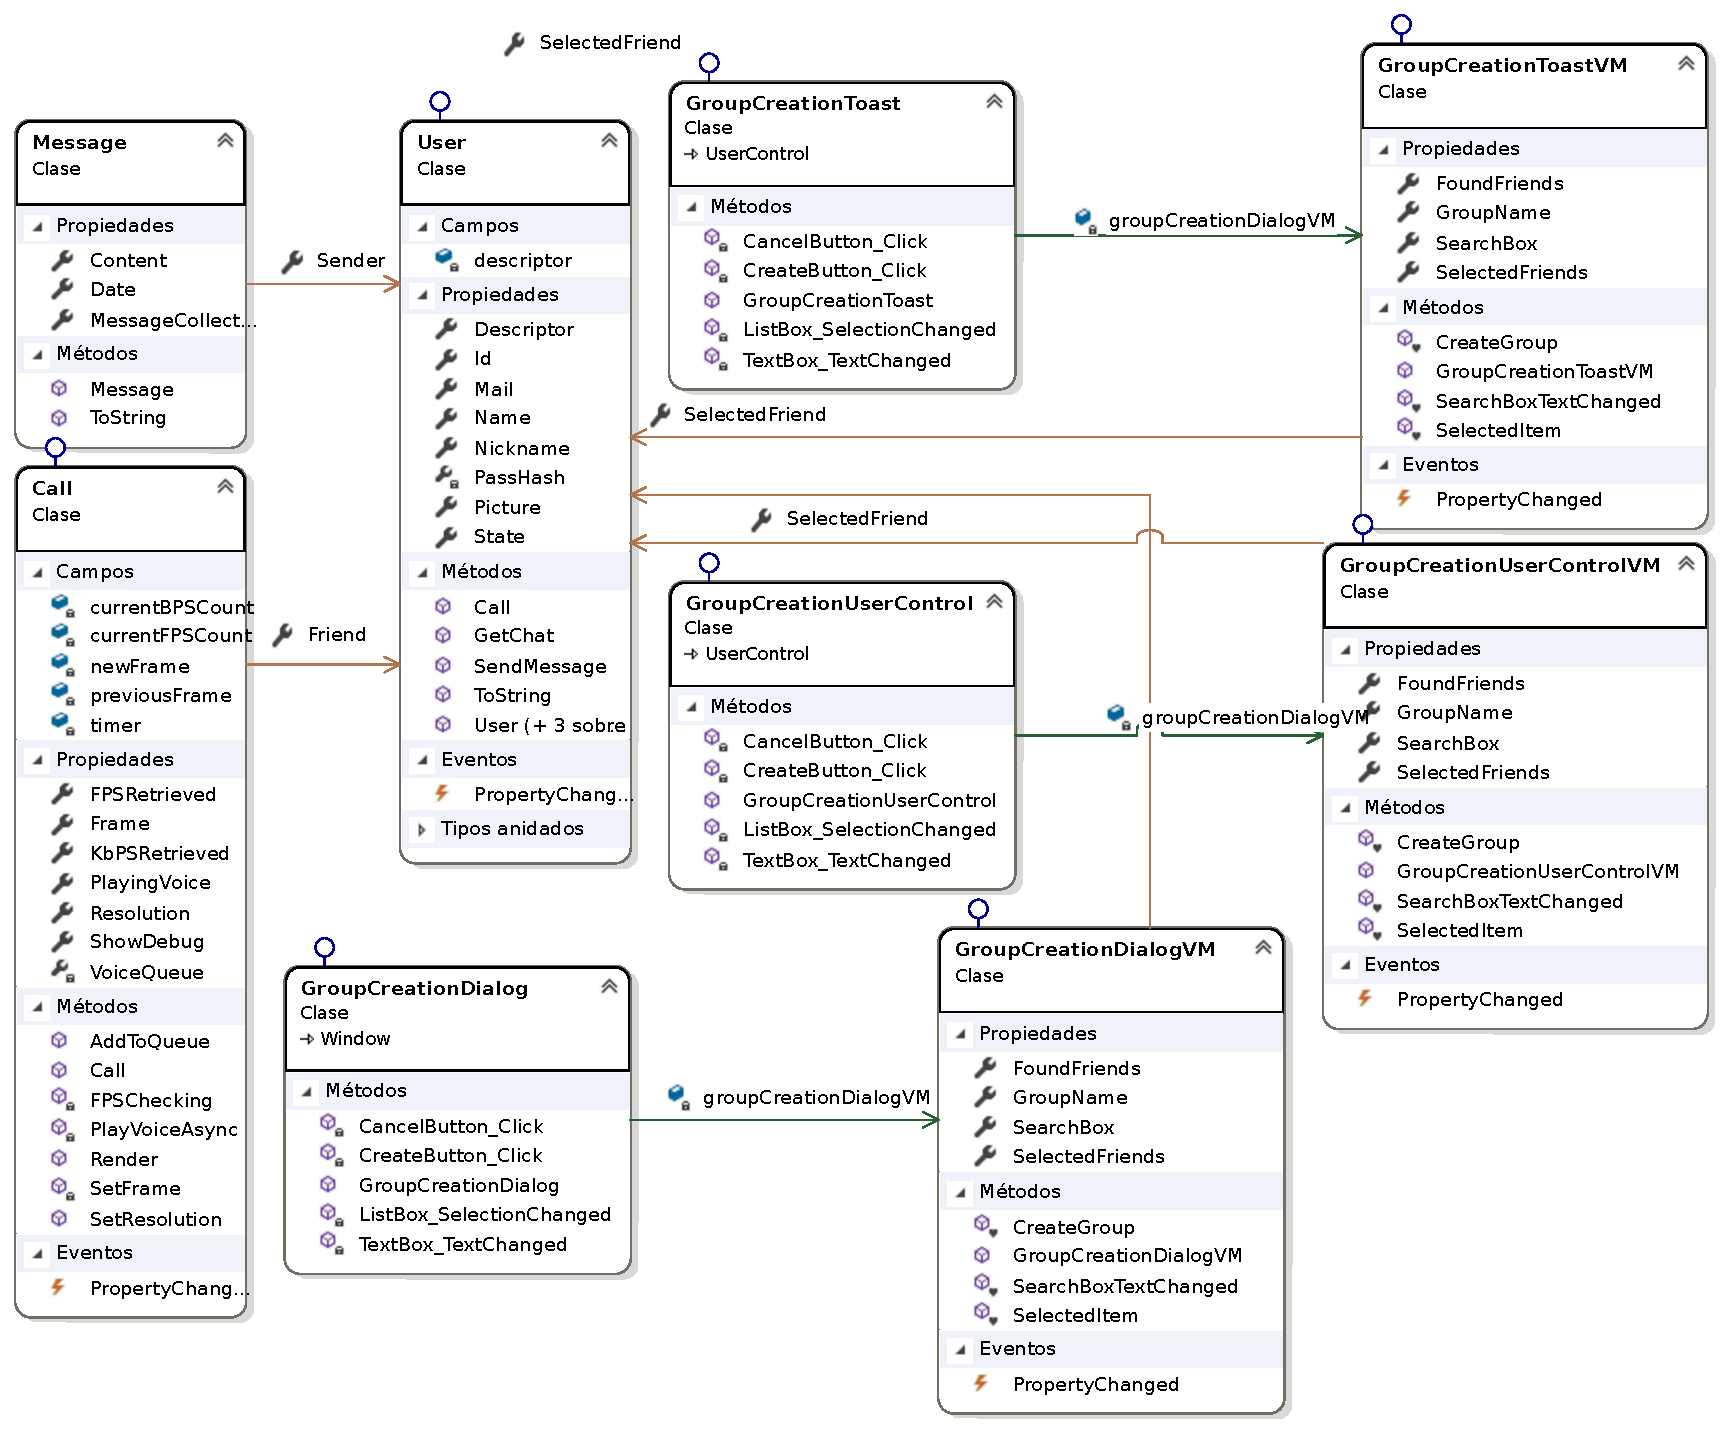
\includegraphics[width=\textwidth,height=\textheight, keepaspectratio]{img/BacoClientDiagram1.pdf}\\
			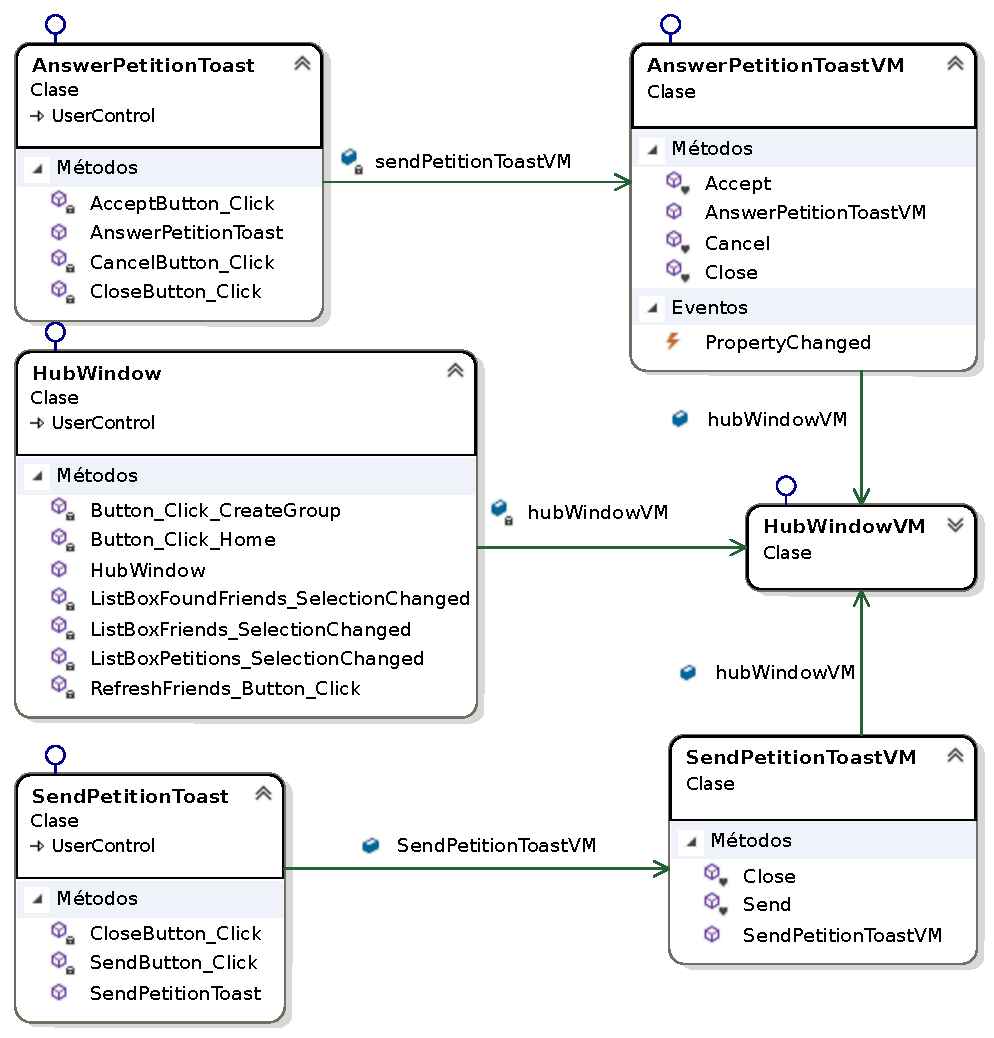
\includegraphics[width=\textwidth,height=\textheight, keepaspectratio]{img/BacoClientDiagram2.pdf}\\
			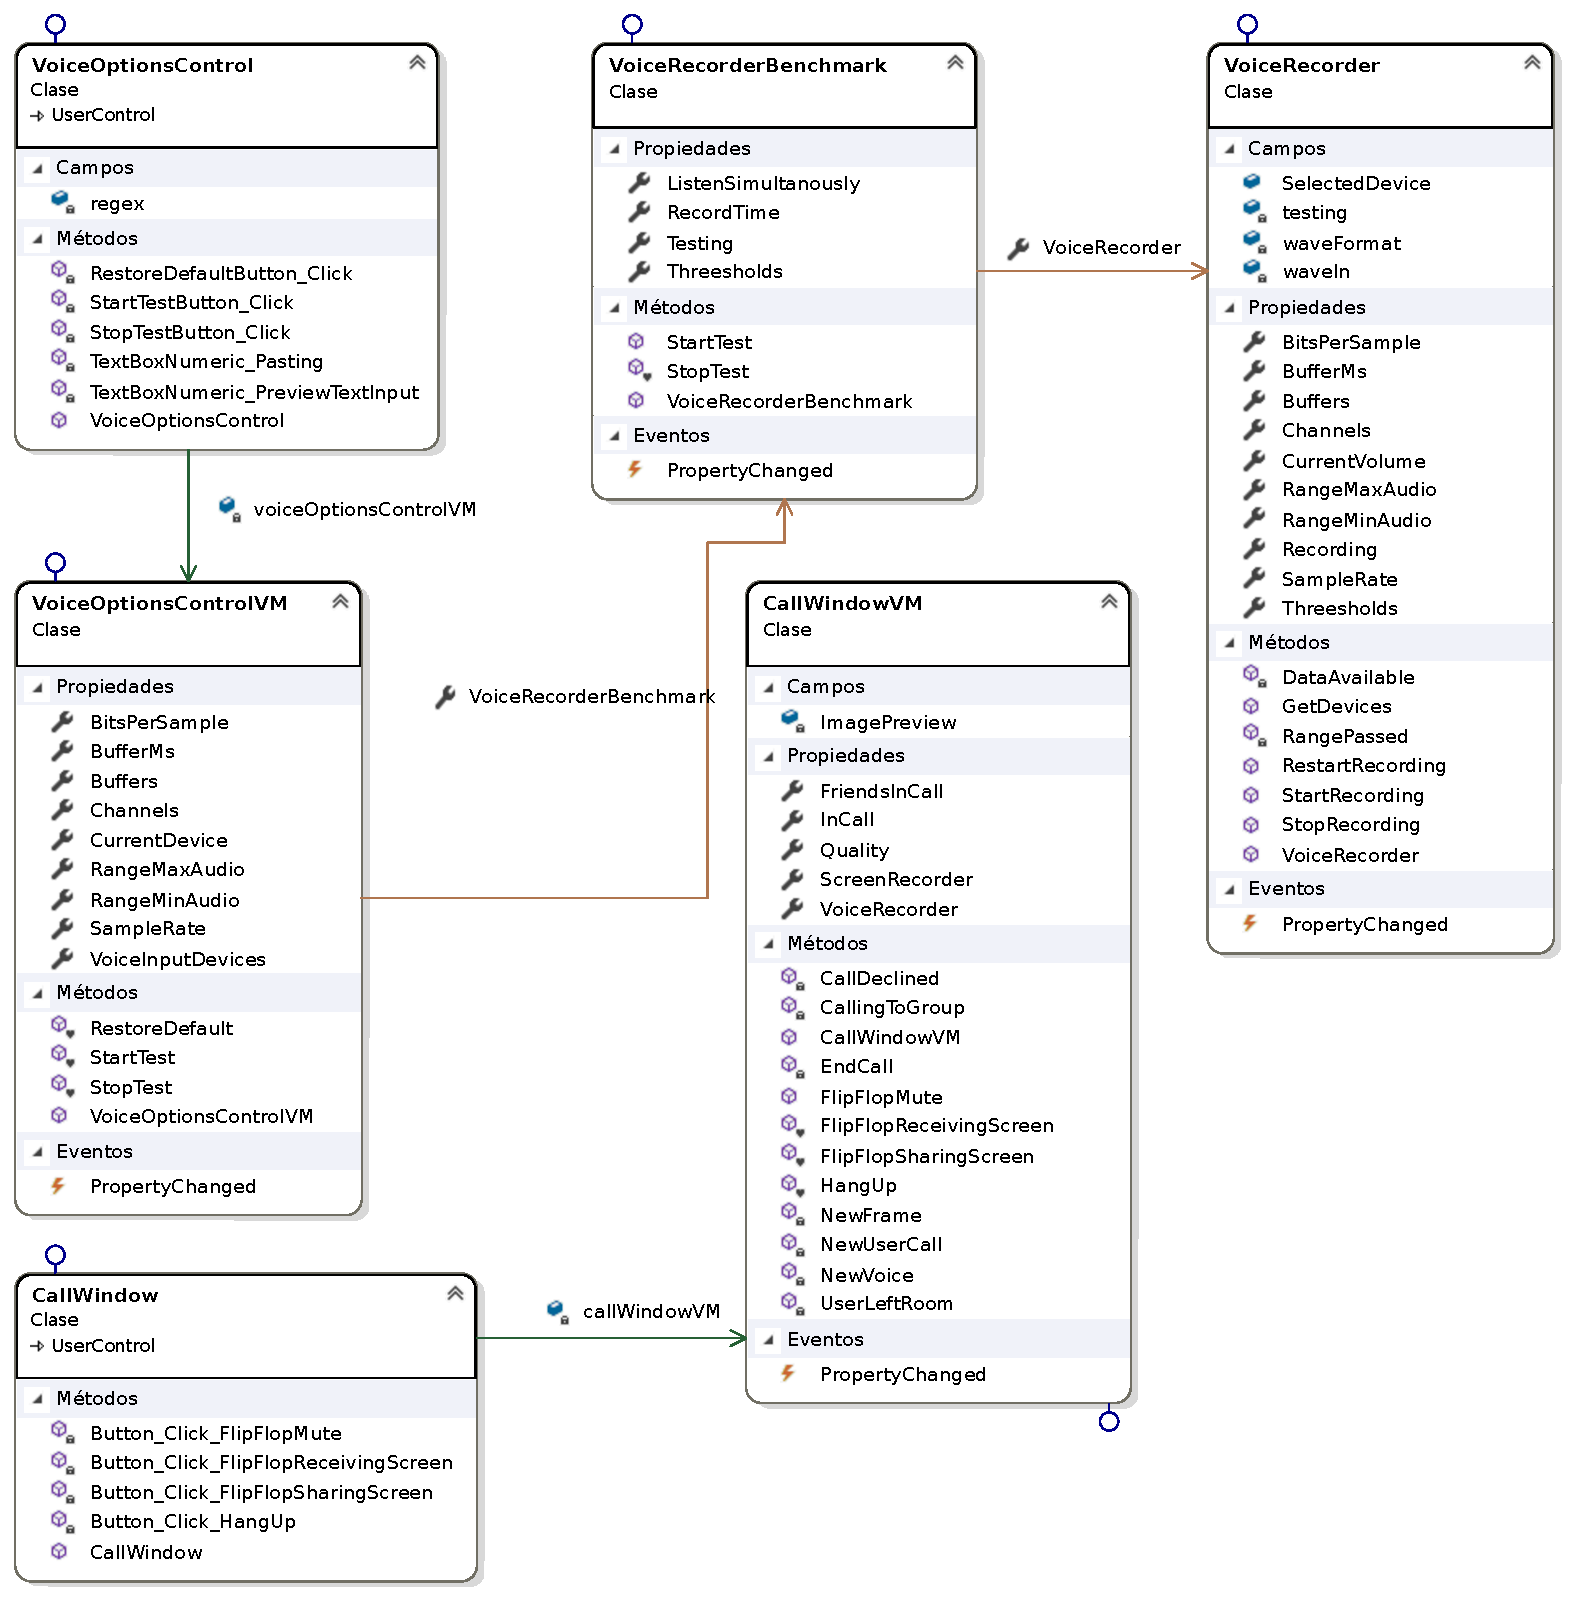
\includegraphics[width=\textwidth,height=\textheight, keepaspectratio]{img/BacoClientDiagram3.pdf}\\
			Debido a que el diagrama es muy extenso no se han incluido las relaciones de colecciones; en el diagrama de a continuación se mostrara completo y con las colecciones, por ello se recomienda ver este documento con un visor de PDF.\\
			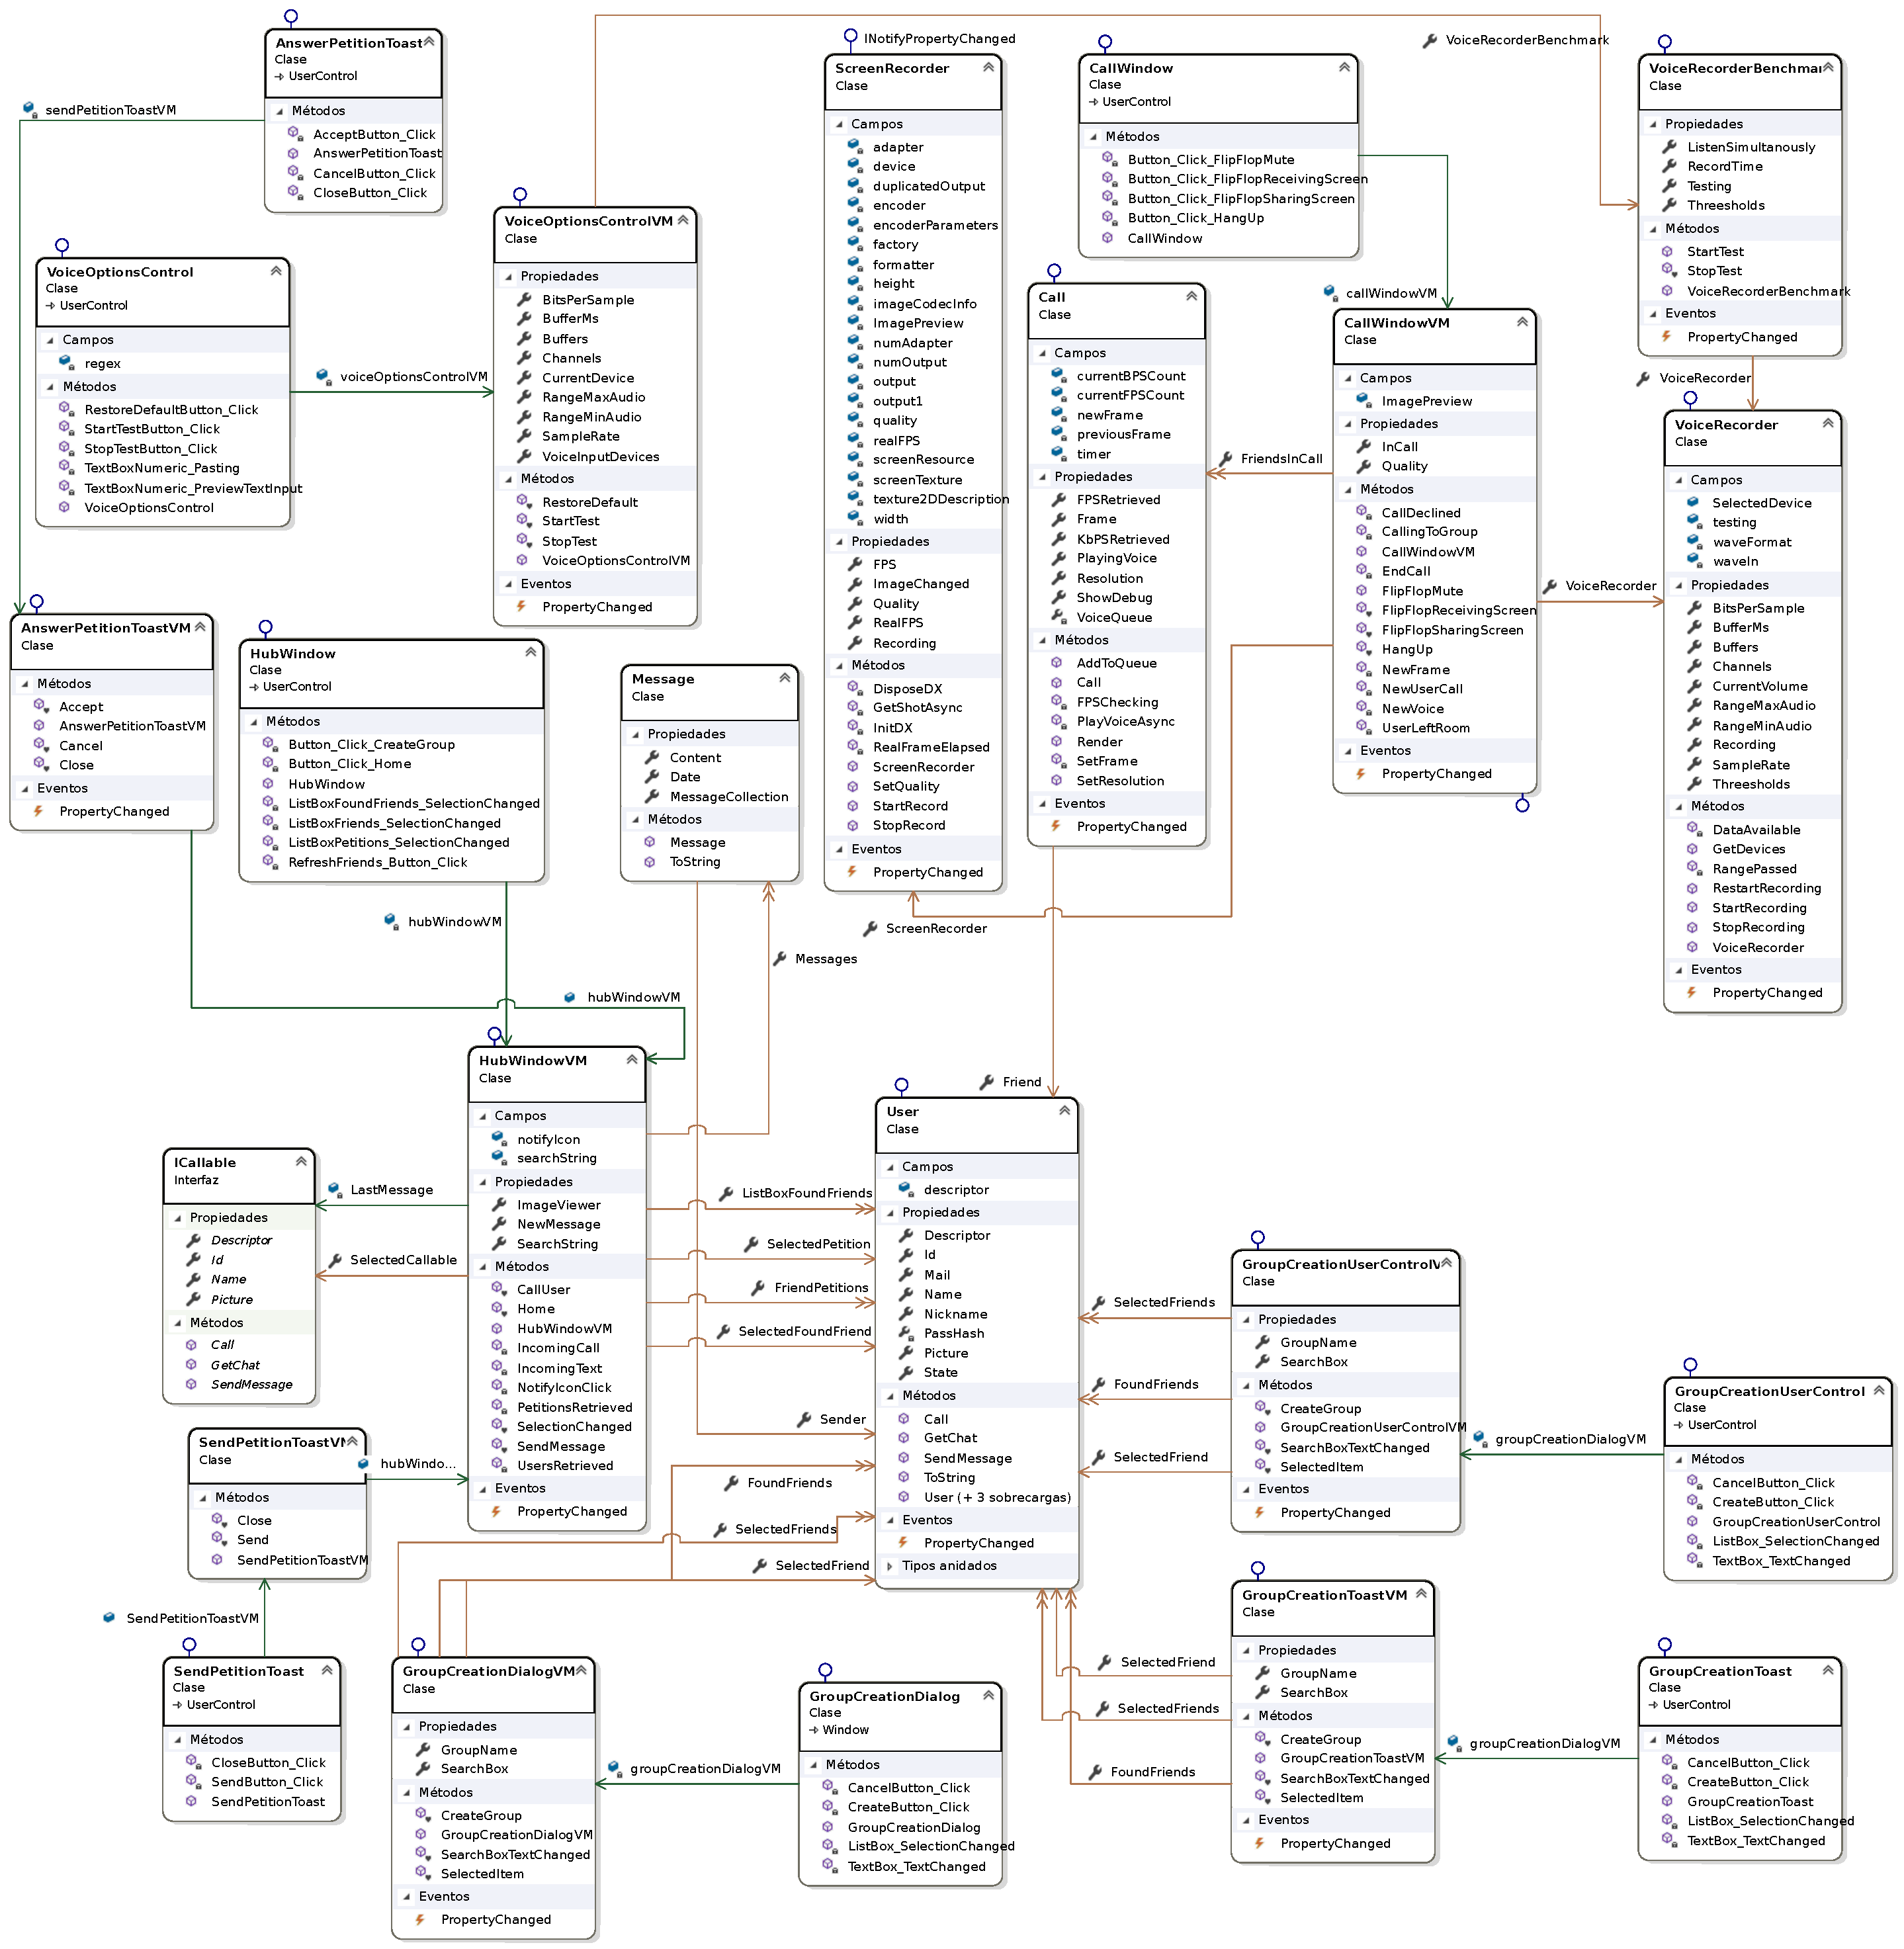
\includegraphics[width=\textwidth,height=\textheight]{img/BacoClientDiagramAll.pdf}\\
			\subsection{Servidor}
			A continuación se muestra el diagrama del servidor.\\
			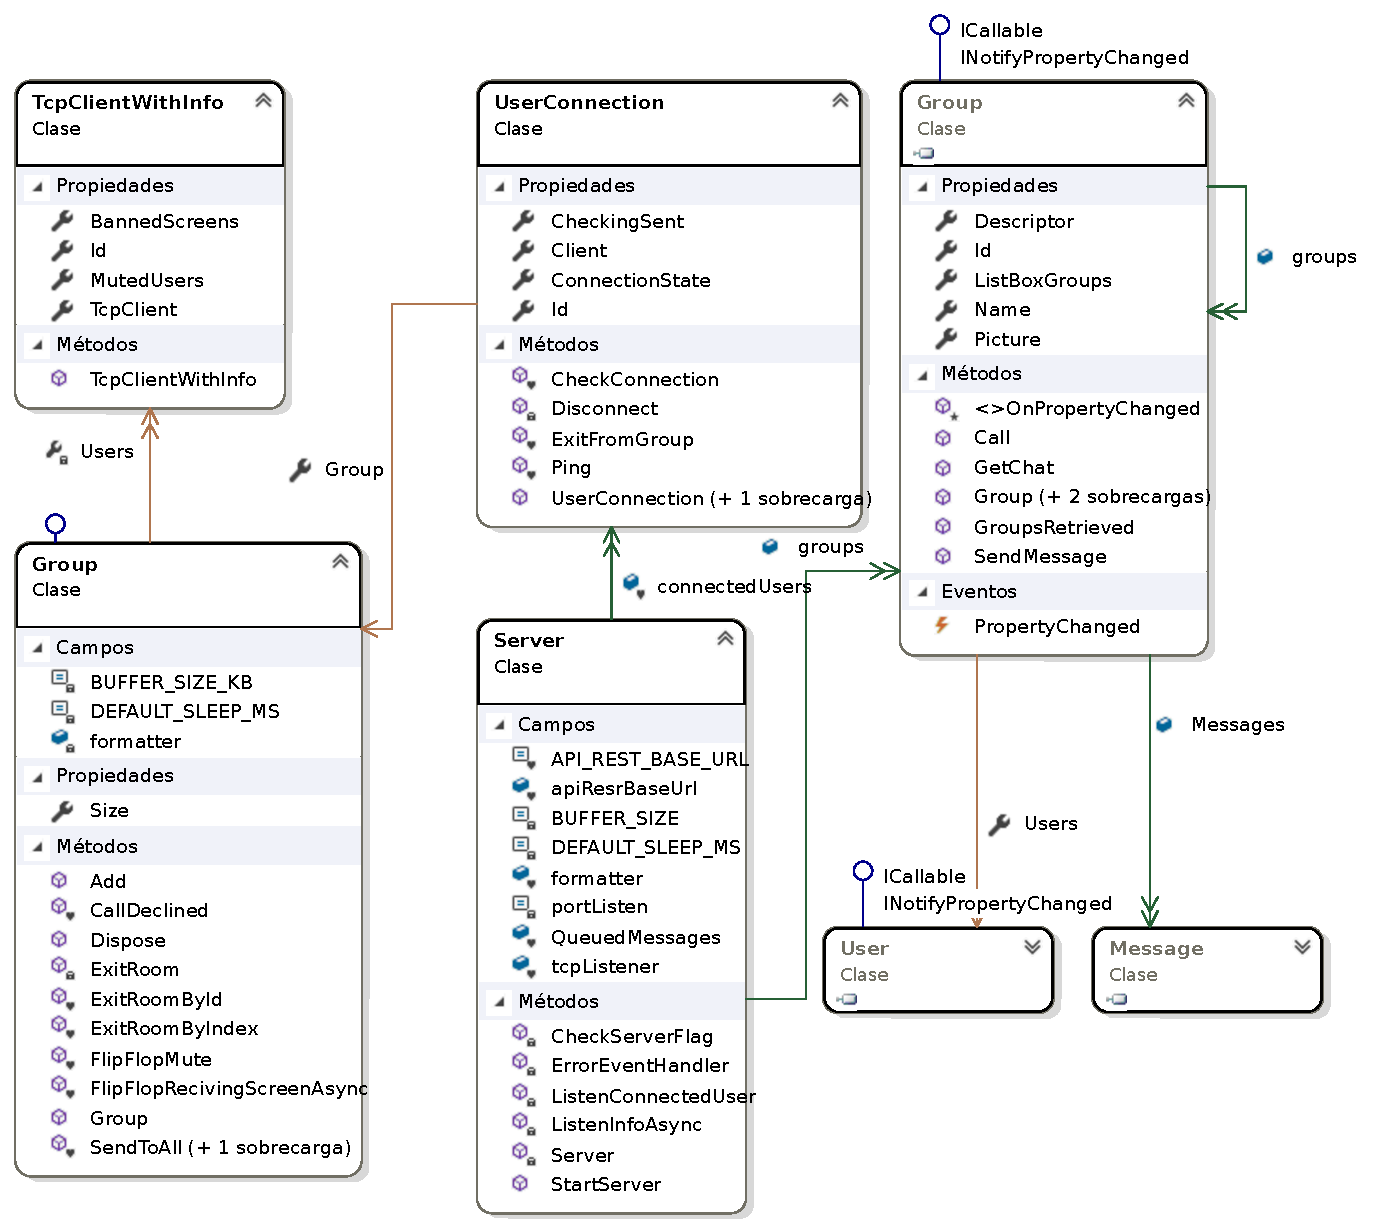
\includegraphics[width=\textwidth,height=\textheight, keepaspectratio]{img/BacoServerDiagram.pdf}\\
%			\newpage

		\section{Diseño de datos}
		Los datos se almacenan en base de datos relacional que se muestra a continuación:\\\\
		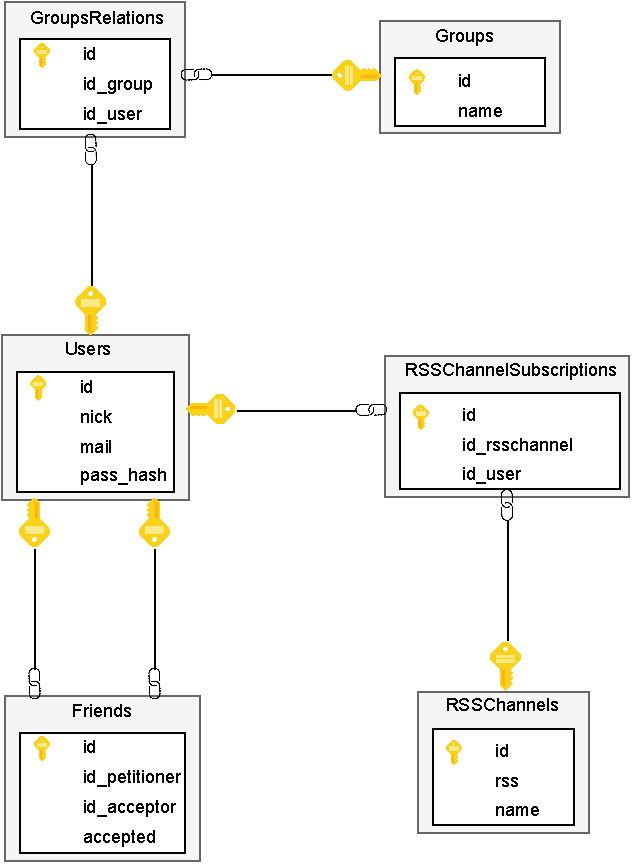
\includegraphics[width=\textwidth,height=\textheight, keepaspectratio]{img/DataDiagram.pdf}\\
		A partir de aquí se hará referencia a las tablas de la base de datos con la siguiente terminología:
		\begin{itemize}
			\item GroupsRelations: relación de de grupos
			\begin{itemize}
				\item id: identificador
				\item id\_group: identificador del grupo
				\item id\_user: identificador del usuario
			\end{itemize}
			\item Groups: grupos
			\begin{itemize}
				\item id: identificador
				\item name: nombre del grupo
			\end{itemize}
			\item Users: usuarios
			\begin{itemize}
				\item id: identificador
				\item nick: nombre de usuario
				\item mail: correo del usuario
				\item pass\_hash: hash de la contraseña del usuario
			\end{itemize}
			\item Friends: amigos
			\begin{itemize}
				\item id: identificador
				\item id\_petitioner: identificador del usuario emisor de la petición
				\item id\_acceptor: identificador del usuario receptor de la petición
				\item accepted: estado de la petición
			\end{itemize}
			\item RSSChannelSubscriptions: suscripciones de canales RSS
			\begin{itemize}
				\item id: identificador
				\item id\_rsschannel: identificador del canal RSS
				\item id\_user: identificador del usuario
			\end{itemize}
			\item RSSChannels: canales RSS
			\begin{itemize}
				\item id: identificador
				\item rss: dirección del canal
				\item name: nombre del canal
			\end{itemize}
		\end{itemize}
		Apréciese en el diagrama la estructura principal de datos donde:
		\begin{itemize}
			\item Un usuario puede tener muchos amigos
			\item Una relación de amistad solo puede tener dos amigos (emisor y receptor)
			\item Un usuario puede tener muchos grupos
			\item Un grupo puede tener muchos usuarios
			\item Un usuario puede tener muchas suscripciones a canales RSS
		\end{itemize}
			\subsection{Amistades}
			Las relaciones de amistad entre usuarios se establecen gracias a la tabla en la base de datos de «amigos». En dicha tabla tenemos dos referencias a los usuarios: quien envía la petición y quien la recibe. El campo que indica el estado de la petición toma tres posibles valores: 1, 0 y nulo, donde:
			\begin{itemize}
				\item 1: aceptada - ambos usuarios son amigos
				\item 0: rechazada - el usuario receptor a rechazado la petición de amistad del emisor
				\item Nulo: sin respuesta - el usuario receptor aún no ha respondido a la petición de amistad
			\end{itemize}
			Debido a este establecimiento de estados nos resulta muy sencillo obtener las peticiones de amistad de cada usuario: si el identificador del usuario en la tabla de amigos tiene como estado «nulo» (siendo el receptor de la petición) sabemos que tiene una petición de amistad (del usuario emisor). Del mismo modo, obtener los amigos de un usuario no es más que buscar tanto en la columna de emisores como la de receptores y obtener el identificador del otro usuario.\\
			Se hablará más adelante de la creación de la base de datos (en la \crthypercref{sbc:db}).
		
	\chapter{Codificación}
	Para la realización de Baco se han requerido diversos entornos, herramientas y lenguajes; todo ello se especificará en las secciones siguientes (\crthypercref{sc:lenguajes}, \crthypercref{sc:entornos}, \crthypercref{sc:herramientas}).
		\section{Lenguajes de programación y marcado} \label{sc:lenguajes}
		Comentaremos los lenguajes que se han usado en los puntos siguientes.
			\subsection{C\#}
			Se ha utilizado C\# para el desarrollo de Baco debido a la familiaridad con este lenguaje.
			\subsection{XAML}
			La interfaz gráfica (\acrshort{gui}) de Baco se ha realizado en WPF, por ello se ha hecho uso de XAML; es un lenguaje de marcado basado en XML y cuya finalidad es definir la GUI de nuestra aplicación.
			\begin{center}
				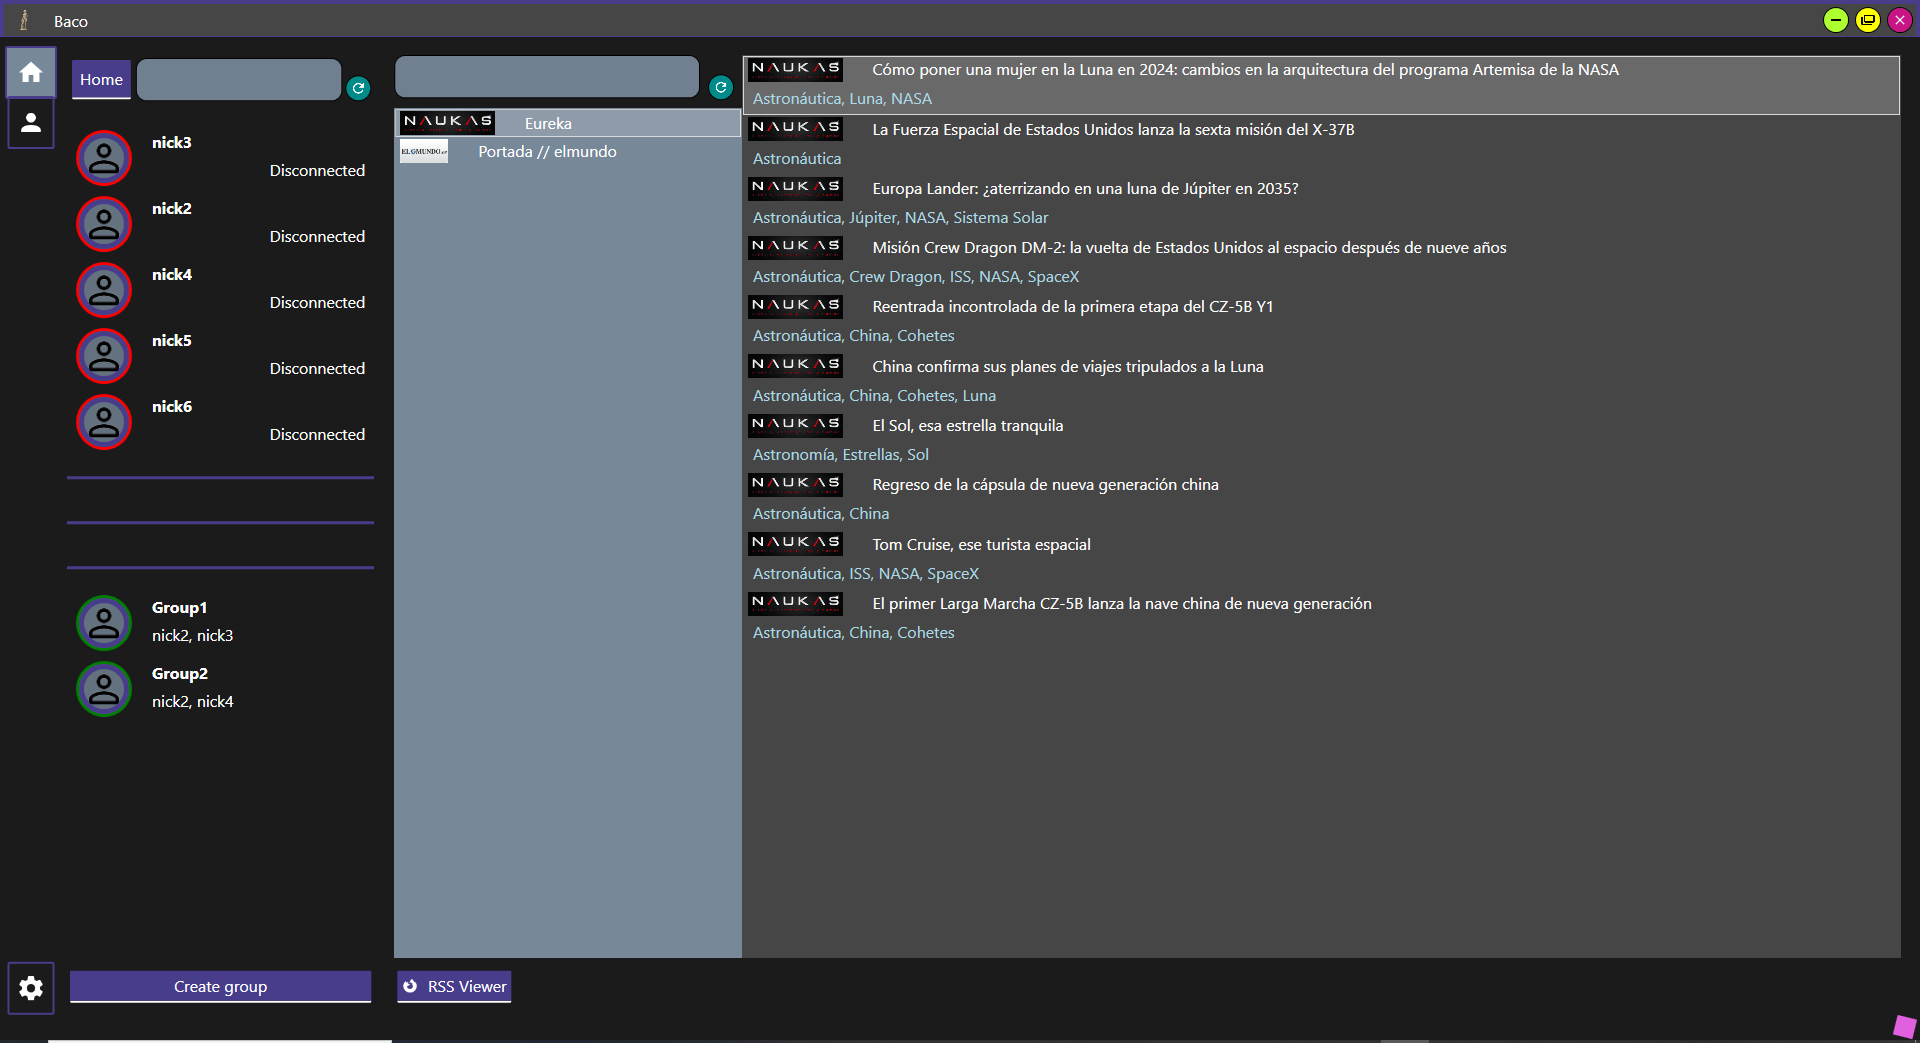
\includegraphics[width=\textwidth,height=\textheight, keepaspectratio]{img/DrawIO/src/hub.PNG}\\
			\end{center}
			\subsection{Transact-SQL (T-SQL)}
			T-SQL es un tipo de lenguaje de consultas estructurado desarrollado por Microsoft; es una extensión de SQL y lo enriquece para incluir diversos aspectos. La principal ventaja es la simplicidad de la exportación de bases de datos a Azure. El por qué de la elección de este lenguaje se especifica en la \crthypercref{sbc:db}.
		\section{Entornos de programación (IDE)} \label{sc:entornos}
		Los entornos han sido elegidos por la cercanía que se tenía a ellos: se habían usado con anterioridad y se tenia un manejo cómodo y con soltura. También se expresarán opiniones personales acerca de ellos.
			\subsection{Visual Studio}
			Visual Studio proporciona herramientas y facilidades (como su \selectlanguage{english}\textit{IntelliSense}\selectlanguage{spanish}) que son superiores a las de sus competidores. Una gran ventaja es la administración de paquetes que este posee (NuGet) el cual comentaremos en el siguiente punto.
				\subsubsection{NuGet}
				A continuación se enumeran los paquetes usados en la solución:\\
				\begin{center}
					\begin{tabular}{|l|c|c|c|c|c|}
						\hline
						\multicolumn{1}{|c|}{Nombre}            	   & Versión & Baco & BacoServer & ApiBaco & Service \\ \hline
						\tiny{Fody}                                    & 6.1.1   & Sí   & No         & No      & No      \\ \hline
						\tiny{Gecko}                                   & 45.0.34 & Sí   & No         & No      & No      \\ \hline
						\tiny{Microsoft.AspNetCore}                    & 2.2.0   & No   & No         & Sí      & No      \\ \hline
						\tiny{Microsoft.AspNetCore.Mvc}                & 2.2.0   & No   & No         & Sí      & No      \\ \hline
						\tiny{Microsoft.AspNetCore.Mvc.Abstractions}   & 2.2.0   & No   & No         & No      & Sí      \\ \hline
						\tiny{Microsoft.Bcl}                           & 1.1.10  & Sí   & No         & No      & No      \\ \hline
						\tiny{Microsoft.Bcl.Build}                     & 1.0.14  & Sí   & No         & No      & No      \\ \hline
						\tiny{\hypertarget{entity}{Microsoft.EntityFrameworkCore}}           & 3.1.2   & No   & No         & Sí      & No      \\ \hline
						\tiny{\hypertarget{entitydesign}{Microsoft.EntityFrameworkCore.Design}}    & 3.1.2   & No   & No         & No      & Sí      \\ \hline
						\tiny{\hypertarget{entityserver}{Microsoft.EntityFrameworkCore.SqlServer}} & 3.1.2   & No   & No         & Sí      & Sí      \\ \hline
						\tiny{\hypertarget{entitytools}{Microsoft.EntityFrameworkCore.Tools}}     & 3.1.2   & No   & No         & Sí      & Sí      \\ \hline
						\tiny{Microsoft.Toolkit}                       & 6.0.0   & Sí   & No         & No      & No      \\ \hline
						\tiny{Microsoft.Toolkit.Parsers}               & 6.0.0   & Sí   & No         & No      & No      \\ \hline
						\tiny{\hypertarget{naudio}{NAudio}}            & 1.10.0  & Sí   & No         & No      & No      \\ \hline
						\tiny{Newtonsoft.Json}                         & 12.0.3  & Sí   & Sí         & No      & No      \\ \hline
						\tiny{PropertyChanged.Fody}                    & 2.6.1   & Sí   & No         & No      & No      \\ \hline
						\tiny{\hypertarget{sharpdx}{SharpDX}}          & 4.2.0   & Sí   & No         & No      & No      \\ \hline
						\tiny{SharpDX.Direct3D11}                      & 4.2.0   & Sí   & No         & No      & No      \\ \hline
						\tiny{SharpDX.DXGI}                            & 4.2.0   & Sí   & No         & No      & No      \\ \hline
						\tiny{System.ServiceModel.Syndication}         & 4.7.0   & No   & Sí         & No      & No      \\ \hline
					\end{tabular}
				\end{center}
			\subsection{SQL Server Management Studio (SSMS)}
			Debido a que T-SQL está desarrollado por Microsoft, el mejor IDE para crear y manejar T-SQL es el SSMS. Provee características para el manejo rápido y sencillo de las bases de datos del sistema: creación y modificación de tablas con una interfaz gráfica, edición de datos de tablas, exportación a Azure sencilla...\\
			Cabe aclarar que no se ha hecho uso de las interfaces gráficas para la creación de las tablas necesarias por Baco, como bien se puede apreciar en la \crthypercref{sbc:db}.
		\section{Herramientas} \label{sc:herramientas}
		Debido a que no solo hacen falta IDE para desarrollar un programa, también cabe mencionar otras herramientas que han sido de utilidad para pruebas. Estos programas se han utilizado exclusivamente para ver y modificar la base de datos.
			\subsection{Mozilla Firefox}
			Se ha hecho uso de Mozilla Firefox por su visor de JSON y para emular la comunicación que Baco tendría con el API REST. A diferencia de Chrome, Firefox viene con un visor JSON incorporado y no requiere de complementos de terceros para ello.
			\subsection{Postman}
			Debido a que los navegadores solo pueden realizar una acción (\selectlanguage{english}\textit{GET}\selectlanguage{spanish}), Postman nos ofrece la posibilidad de enviar datos a nuestro API REST con acciones como \selectlanguage{english}\textit{UPDATE}\selectlanguage{spanish}, \selectlanguage{english}\textit{PUT}\selectlanguage{spanish} o \selectlanguage{english}\textit{POST}\selectlanguage{spanish}. Si bien es cierto que Postman podría hacer ek trabajo de Mozilla Firefox, este es más cómodo de manejar debido a que es un navegador web (es decir, no te da tantas opciones para enviar al servidor como Postman).
		\section{Aspectos relevantes de la implementación}
		A continuación, se expondrán y comentarán fragmentos de código de difícil comprensión. Entiéndase por <<difícil comprensión>> aquellos fragmentos que queden fuera de los conocimientos adquiridos.
			\subsection{API}
			El API REST esta realizado en C\#, .NET Core 3.1. Consta de dos proyectos: ApiBaco (\crthypercref{sbc:api}) y Service (\crthypercref{sbc:service}).
				\subsubsection{ApiBaco} \label{sbc:api}
				Es una aplicación de consola que recibe las peticiones HTTP y envía los datos solicitados. Para la realización de este se ha tenido que estudiar como se comporta en C\# \cite{Learn_Entity_Framework_Core}.
				\subsubsection{Service} \label{sbc:service}
				Es una librería de clases; aquí es donde reside la comunicación con la base de datos. Este proyecto es quien posee la lógica respecto al acceso a datos. El proyecto ApiBaco (\crthypercref{sbc:api}) llama a las funciones que este posee.
			\subsection{Cliente -- Baco}
			Pese a la magnitud del proyecto Baco, su composición es relativamente simple; se quieren matizar las siguientes clases debido a que su nivel de complejidad puede dar lugar a la no comprensión de la finalidad. También se explicará cómo se envía la pantalla por llamada.
				\subsubsection{ScreenRecorder.cs}
				\selectlanguage{english}\textit{ScreenRecorder}\selectlanguage{spanish} es la clase encargada de capturar y enviar la pantalla. Dicha acción se realiza haciendo uso de DirectX mediante el paquete \hyperlink{sharpdx}{SharpDX}.\\
				Vamos a explicar de forma rápida cómo se graba y envía el vídeo. Para comenzar, empezaremos por la función encargada de empezar a grabar:
				\lstinputlisting[language=csh,basicstyle=\scriptsize,firstline=278,lastline=301,caption={Inicio de grabaci\'{o}n de pantalla}]{../Baco/Recorder/ScreenRecorder.cs}
				Nada más iniciar la función, la línea \hyperlink{../Baco/Recorder/ScreenRecorder.cs280}{280} comprueba si se está grabando ya la pantalla; en caso contrario se procederá a comenzar a grabar. Desde la línea \hyperlink{../Baco/Recorder/ScreenRecorder.cs282}{282} hasta la \hyperlink{../Baco/Recorder/ScreenRecorder.cs287}{287} se configura el <<temporizador>> que va a ser nuestro contador de FPS reales. El temporizador ejecutará cada segundo la función que actualizará los FPS reales. Establecemos cuál será el control encargado de la previsualización de la captura y dejamos corriendo en un hilo la grabación. En el bucle de la línea \hyperlink{../Baco/Recorder/ScreenRecorder.cs293}{293} tenemos tres líneas; la primera accede a la función encargada de grabar y enviar la captura (), la segunda se espera el tiempo necesario entre captura y captura y por último añadimos uno al contador de FPS reales.\\
				La captura de pantalla se lleva a cabo con la función <<\selectlanguage{english}\textit{GetShotAsync}\selectlanguage{spanish}>>:
				\lstinputlisting[language=csh,basicstyle=\scriptsize,firstline=156,lastline=270,caption={Grabaci\'{o}n de pantalla y env\'{i}o de v\'{i}deo}]{../Baco/Recorder/ScreenRecorder.cs}
				La función de grabación y emisión de vídeo tiene lugar de la línea \hyperlink{../Baco/Recorder/ScreenRecorder.cs160}{160} a la \hyperlink{../Baco/Recorder/ScreenRecorder.cs226}{226}, y en ellas se aprecian las siguientes partes:
				\hspace*{2cm}
				\begin{itemize}
					\item \hyperlink{../Baco/Recorder/ScreenRecorder.cs160}{160} -- \hyperlink{../Baco/Recorder/ScreenRecorder.cs174}{174}: definición de cómo será la imagen capturada. Se obtienen las dimensiones de la pantalla para la captura y se copia la textura de la pantalla a memoria; la textura se extrae del objeto <<\selectlanguage{english}\textit{device}\selectlanguage{spanish}>> (que aparece por primera vez en la línea \hyperlink{../Baco/Recorder/ScreenRecorder.cs169}{169}) y se copia a otro objeto el cuál sabremos en todo momento dónde está (el objeto <<\selectlanguage{english}\textit{device}\selectlanguage{spanish}>> podría cambiar su valor en cualquier momento). Y las últimas dos líneas dejan predefinido cómo tendrán que ser los datos más básicos de la imagen.
					\item \hyperlink{../Baco/Recorder/ScreenRecorder.cs180}{180} -- \hyperlink{../Baco/Recorder/ScreenRecorder.cs197}{197}: Creación de la imagen y liberación de la GPU. La primera instrucción especifica los atributos de la imagen resultante de la captura de pantallas y las dos siguientes nos harán falta para copiar en memoria de forma rápida la captura en forma de mapa de bits. El bucle que sigue será el encargado de ir de fila en fila de la imagen capturada e irá copiándose en memoria las filas que lea. Fura del bucle, en la línea \hyperlink{../Baco/Recorder/ScreenRecorder.cs195}{195}, se desbloquea el mapa de bits con los atributos especificados y la línea siguiente libera el recurso que accede a la captura de pantalla por parte de la GPU; por ello, en el punto superior se comentaba que <<\selectlanguage{english}\textit{device}\selectlanguage{spanish}>> puede cambiar de valor en cualquier momento. Dado que esto está sucediendo en un hilo a parte, otro hilo puede ahora acceder al objeto <<\selectlanguage{english}\textit{device}\selectlanguage{spanish}>> y realizar, a la vez, las mismas acciones que estamos en este momento realizando.
					\item \hyperlink{../Baco/Recorder/ScreenRecorder.cs201}{201} -- \hyperlink{../Baco/Recorder/ScreenRecorder.cs223}{223}: compresión de imagen, previsualización y envío. La primera línea almacena en un \selectlanguage{english}\textit{stream}\selectlanguage{spanish} de memoria el mapa de bits resultante de las acciones anteriores y lo comprime con los códecs y los parámetros de envío. La imagen comprimida es mostrada en la línea \hyperlink{../Baco/Recorder/ScreenRecorder.cs211}{211}. La siguiente instrucción (concretamente la función de la clase <<\selectlanguage{english}\textit{VideoFrame}\selectlanguage{spanish}>>) se encarga de:
					\begin{enumerate}
						\item Cortar la imagen en porciones iguales.
						\item Comparar las porciones con las porciones de la imagen anterior (si no existe imagen anterior no se compararán).
						\item Determinar qué porciones son las que han cambiado.
						\item Devolver una lista con, únicamente, las porciones de la imagen que han cambiado.
					\end{enumerate}
					Al enviar únicamente las porciones que cambian reducimos considerablemente el uso de red cuando se envía la pantalla, llegando a darse casos de 0 Kb/s en momentos en los que la pantalla no se mueve. La función que realiza las particiones emplea una algoritmia basada en probabilidades, se estima la probabilidad de que una fragmento haya cambiado con respecto al anterior, por ejemplo: dado el caso de una retransmisión de vídeo supongamos que el emisor del vídeo retransmite un vídeo; la pantalla que se transmite es la siguiente:\\
					\begin{center}
						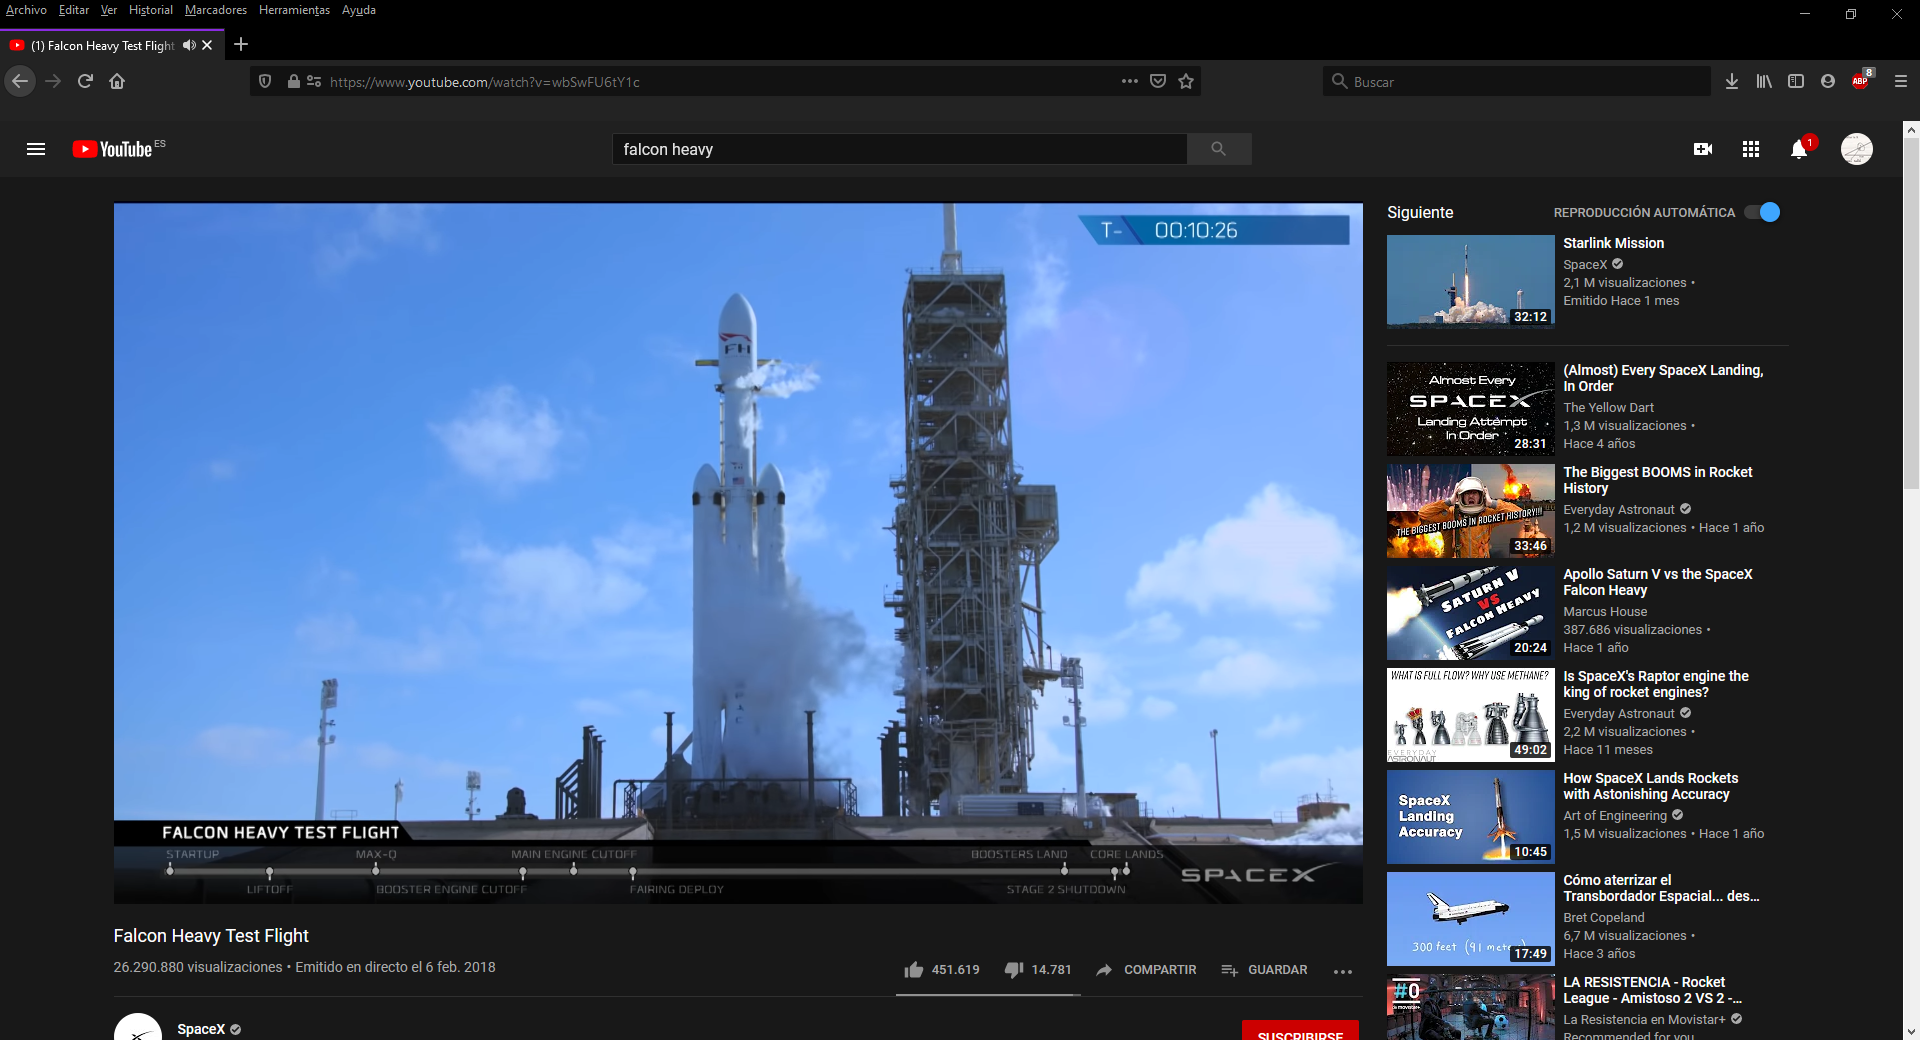
\includegraphics[width=\textwidth,height=\textheight, keepaspectratio]{img/DrawIO/src/videoemission.PNG}\\
					\end{center}
					Como podremos suponer, en la zona del vídeo es dónde, principalmente, sucederán los cambios. En la siguiente imagen se resalta:\\
					\begin{center}
						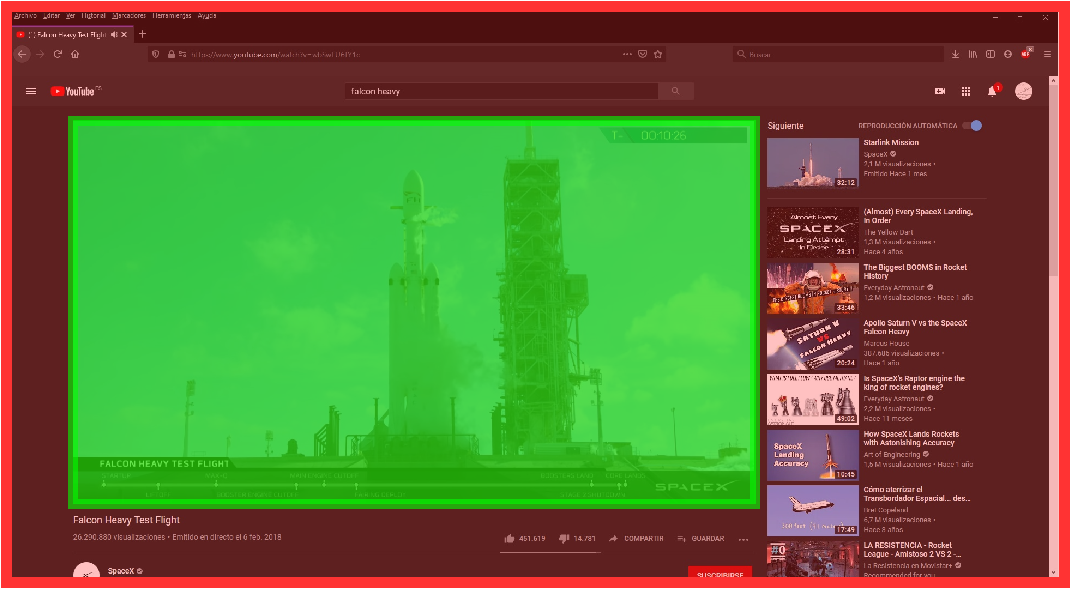
\includegraphics[width=\textwidth,height=\textheight, keepaspectratio]{img/VideoEmission.pdf}\\
					\end{center}
					Véase la zona coloreada en verde como los fragmentos que más probabilidad tienen de cambiar y los rojos los que menos. En este supuesto, si el usuario no se desplaza por la página, solamente se enviará la zona sombreada en verde, que es la zona que va a cambiar, el resto de las zonas (la parte sombreada en rojo) no se van a comprobar todas para ver si hay cambios, solamente algunas dado que la probabilidad de que haya algún cambio en ella es baja.\\
					En el supuesto de que no haya ningún cambio se retorna un valor nulo. Dicho valor nulo nos servirá para, en la línea \hyperlink{../Baco/Recorder/ScreenRecorder.cs217}{217}, enviar o no la pantalla; evidentemente, si no hay cambios no se envía nada. En el caso de haberlos se comprime la lista en memoria junto con la especificación de las dimensiones de la pantalla (línea \hyperlink{../Baco/Recorder/ScreenRecorder.cs221}{221}), de este modo sabremos cuál es la posición de cada bloque que enviamos con respecto a la resolución. Por último se envía el objeto serializado en memoria al servidor para que él lo retransmita a los usuarios de la llamada (solo a aquellos que estén viendo la retransmisión).
				\end{itemize}
				\subsubsection{VoiceRecorder.cs}
				La clase \selectlanguage{english}\textit{VoiceRecorder}\selectlanguage{spanish} detecta los dispositivos de entrada de audio y captura el sonido para ser enviado por red o para hacer pruebas de sonido (en el menú de opciones). El paquete que hace esto posible es \hyperlink{naudio}{NAudio}.\\
				Funciona de un modo similar a la clase ScreenRecorder.cs, solo que en vez de capturar la pantalla lee el voltaje del dispositivo de entrada de audio. Esto sucede en la siguiente función:
				\lstinputlisting[language=csh,basicstyle=\scriptsize,firstline=59,lastline=72,caption={Inicio de captura de micr\'{o}fono}]{../Baco/Recorder/VoiceRecorder.cs}
				La primera línea nos permite determinar cómo vamos a transformar la señal analógica del micrófono a su señal digital. A continuación, en las líneas que van de la \hyperlink{../Baco/Recorder/VoiceRecorder.cs62}{62} a la \hyperlink{../Baco/Recorder/VoiceRecorder.cs68}{68}, se establecen los parámetros que indican como se ha de capturar la información del micrófono:
				\begin{enumerate}
					\item El búfer: cuánto tiempo se va guardar en el búfer.
					\item El dispositivo de entrada: indicará el índice del dispositivo a leer.
					\item Formato de la modulación por impulsos codificados: lo comentado anteriormente, cómo se va a transformar la señal analógica en digital.
					\item Número de búferes: cuántos búferes se usarán.
				\end{enumerate}
				Antes de comenzar a leer en la línea \hyperlink{../Baco/Recorder/VoiceRecorder.cs70}{70}, la instrucción anterior es la suscripción al evento <<\selectlanguage{english}\textit{DataAvailable}\selectlanguage{spanish}>>. Este evento se lanza cada vez que se llene el búfer que hayamos especificado y será donde se envíe el audio. La función suscrita es la siguiente:
				\lstinputlisting[language=csh,basicstyle=\scriptsize,firstline=98,lastline=121,caption={B\'{u}fer de lectura lleno}]{../Baco/Recorder/VoiceRecorder.cs}
				Primeramente nos encontramos una condición para enviar el audio; dicha condición supondrá si el audio disponible en el búfer está en el rango de volumen para ser enviado (el sonido no es ni muy alto ni muy bajo). En el caso de estarlo se comprueba si el dispositivo de entrada ha cambiado, si no, se comprime (serializando) el audio. Antes de ser enviado el audio comprimido se comprueba si se está en llamada o se está haciendo pruebas en el menú de opciones. Si se están haciendo pruebas, el sonido se reproduce por el dispositivo de salida del propio ordenador, si no se están haciendo pruebas se envía al servidor para su retransmisión a los que estén escuchando al usuario en la llamada.
			\subsection{Servidor -- BacoServer}
			Debido a que el servidor actúa principalmente a modo de pasarela, no se ve necesario ninguna explicación del código. También es el encargado de tener un registro de los usuarios que están conectados en cada momento y manejar las llamadas.
			\subsection{Base de datos} \label{sbc:db}
			Dada la elección de base de datos de Microsoft SQL se ha tenido que implementar la base de datos en su lenguaje nativo: T-SQL. Microsoft SQL nos permite la exportación a objetos desde la base de datos a nuestra solución por medio de la consola del administrador de paquetes NuGet. Hacen falta los paquetes de \hyperlink{entity}{Microsoft.EntityFrameworkCore}, \hyperlink{entitydesign}{Microsoft.EntityFrameworkCore.Design}, \hyperlink{entityserver}{Microsoft.EntityFrameworkCore.SqlServer} y \hyperlink{entitytools}{Microsoft.EntityFrameworkCore.Tools}. Tan solo es necesario un comando tanto como para crear como para actualizar:
			\begin{center}
				\textsf{Scaffold-DbContext ``Server=\textbf{DirecciónInstancia}; Database=\textbf{NombreDB}; Trusted\slash Connection=True;'' Microsoft.EntityFrameworkCore.SqlServer -OutputDir \textbf{CarpetaSalida} -Context ``\textbf{NombreContexto}'' -DataAnnotations}
			\end{center}
			En mi caso, dado:
			\begin{itemize}
				\item \textbf{DirecciónInstancia}: localhost\slash SQLEXPRESS05
				\item \textbf{NombreDB}: baco
				\item \textbf{CarpetaSalida}: Model
				\item \textbf{NombreContexto}: BacoContext
			\end{itemize}
			tendríamos el comando de la siguiente manera:
			\begin{center}
				\textsf{Scaffold-DbContext ``Server=\textbf{localhost\slash SQLEXPRESS05}; Database=\textbf{baco}; Trusted\_Connection=True;'' Microsoft.EntityFrameworkCore.SqlServer -OutputDir \textbf{Model} -Context ``\textbf{BacoContext}'' -DataAnnotations}
			\end{center}
			En el caso de querer actualizar el proyecto con la base de datos solo tendríamos que añadir el parámetro ``-Force'':
			\begin{center}
				\hypertarget{updatestring}{\textsf{Scaffold-DbContext ``Server=\textbf{localhost\slash SQLEXPRESS05}; Database=\textbf{baco}; Trusted\_Connection=True;'' Microsoft.EntityFrameworkCore.SqlServer -OutputDir \textbf{Model} -Context ``\textbf{BacoContext}'' -DataAnnotations -Force}}
			\end{center}
			Una vez realizado el comando sobre un proyecto (en nuestro caso «Service») nos quedaría una estructura de directorios como esta:\\
			\hypertarget{servicetree}{\dirtree{%
					.1 Service.
					.2 Model\DTcomment{Carpeta autogenerada por el \hyperlink{updatestring}{comando de mapeo}}.
					.3 \hypertarget{bacocontext}{BacoContext.cs}\DTcomment{Contexto sobre el cual se accede a los datos}.
					.3 Friends.cs.
					.3 Groups.cs.
					.3 GroupsRelations.cs.
					.3 Rsschannels.cs.
					.3 RsschannelSubscriptions.cs.
					.3 Users.cs.
			}}
			donde \hyperlink{bacocontext}{BacoContext.cs} es el contexto con el cual vamos a acceder a la base de datos. El resto de objetos son los que nos ha mapeado automáticamente Microsoft.EntityFrameworkCore y los cuales se usarán para recibir los datos del contexto.\\
			Para el acceso a los datos en Baco se ha decidido que el proyecto \hyperlink{servicetree}{Service} sea una biblioteca de clases. A dicha biblioteca accede el proyecto ApiBaco. ApiBaco es el servicio REST de nuestro proyecto; haciendo uso de la librería Service es capaz de acceder a la base de datos.\\
			La disposición de datos (cliente y API REST) nos permite tener todo en una misma máquina (no obstante podría soportar estar en máquinas separadas el API REST y el servidor).\\
			Puesto que no se ha impartido el lenguaje se va a mostrar el código necesario para la creación de la base de datos con valores de pruebas:
			\lstinputlisting[language=sql,basicstyle=\scriptsize, caption={Script T-SQL de creaci\'{o}n de la base de datos de Baco}]{src/baco.sql}
			Hasta la línea \hyperlink{src/baco.sql51}{51} el script se encarga de la creación de las tablas base de datos. Véase que T-SQL es igual de SQL. De ahí hasta el final es la inserción de datos a las tablas creadas.\\
			Se ha querido plasmar el código T-SQL para demostrar que no posee diferencias notables respecto a SQL.\\
			Puesto que la base de datos está alojada en el ordenador personal, la versión final habría de ser exportada a una base de datos como Azure. Para ello se hará uso de \href{https://www.microsoft.com/en-us/download/confirmation.aspx?id=53595}{Microsoft Data Migration Assistant}. Una vez se ha hecho la migración, para conectarla con nuestro servicio tan solo habría que actualizar como se hizo en la \hyperlink{updatestring}{cadena de actualización de servicio} pero con ligeros cambios:
			\begin{center}
				\textsf{Scaffold-DbContext ``Server=\textbf{URLAzure};Database=\textbf{NombreAzureDB};User Id=\textbf{Usuario};Password=\textbf{Contraseña}'' Microsoft.EntityFrameworkCore.SqlServer -OutputDir \textbf{CarpetaSalida} -Context ``\textbf{NombreContexto}'' -DataAnnotations -Force}
			\end{center}
			En mi caso seria la siguiente cadena:
			\begin{center}
				\textsf{Scaffold-DbContext ``Server=\textbf{dbcarlosclement.database.windows.net};Database=\textbf{BacoDB};User Id=\textbf{administrador};Password=\textbf{\#admin123}'' Microsoft.EntityFrameworkCore.SqlServer -OutputDir \textbf{Model} -Context ``\textbf{BacoContext}'' -DataAnnotations -Force}
			\end{center}
	\chapter{Manuales de usuario} \label{ch:man}
	Debido a que se han entregado dos proyectos con instaladores se ha procedido a elaborar dos manuales de usuario: el de cliente y el del servidor. El servidor también tiene un manual dado que las empresas pueden interesarse por tener un servidor privado.\\
	Los manuales se anexan a escala 0.75; si se quieren ver a escala 1 estos manuales están incluidos en los ficheros entregados. 
		\section{Baco}
		Anexado en esta sección se encuentra el manual de usuario de Baco.
		\cleardoublepage
		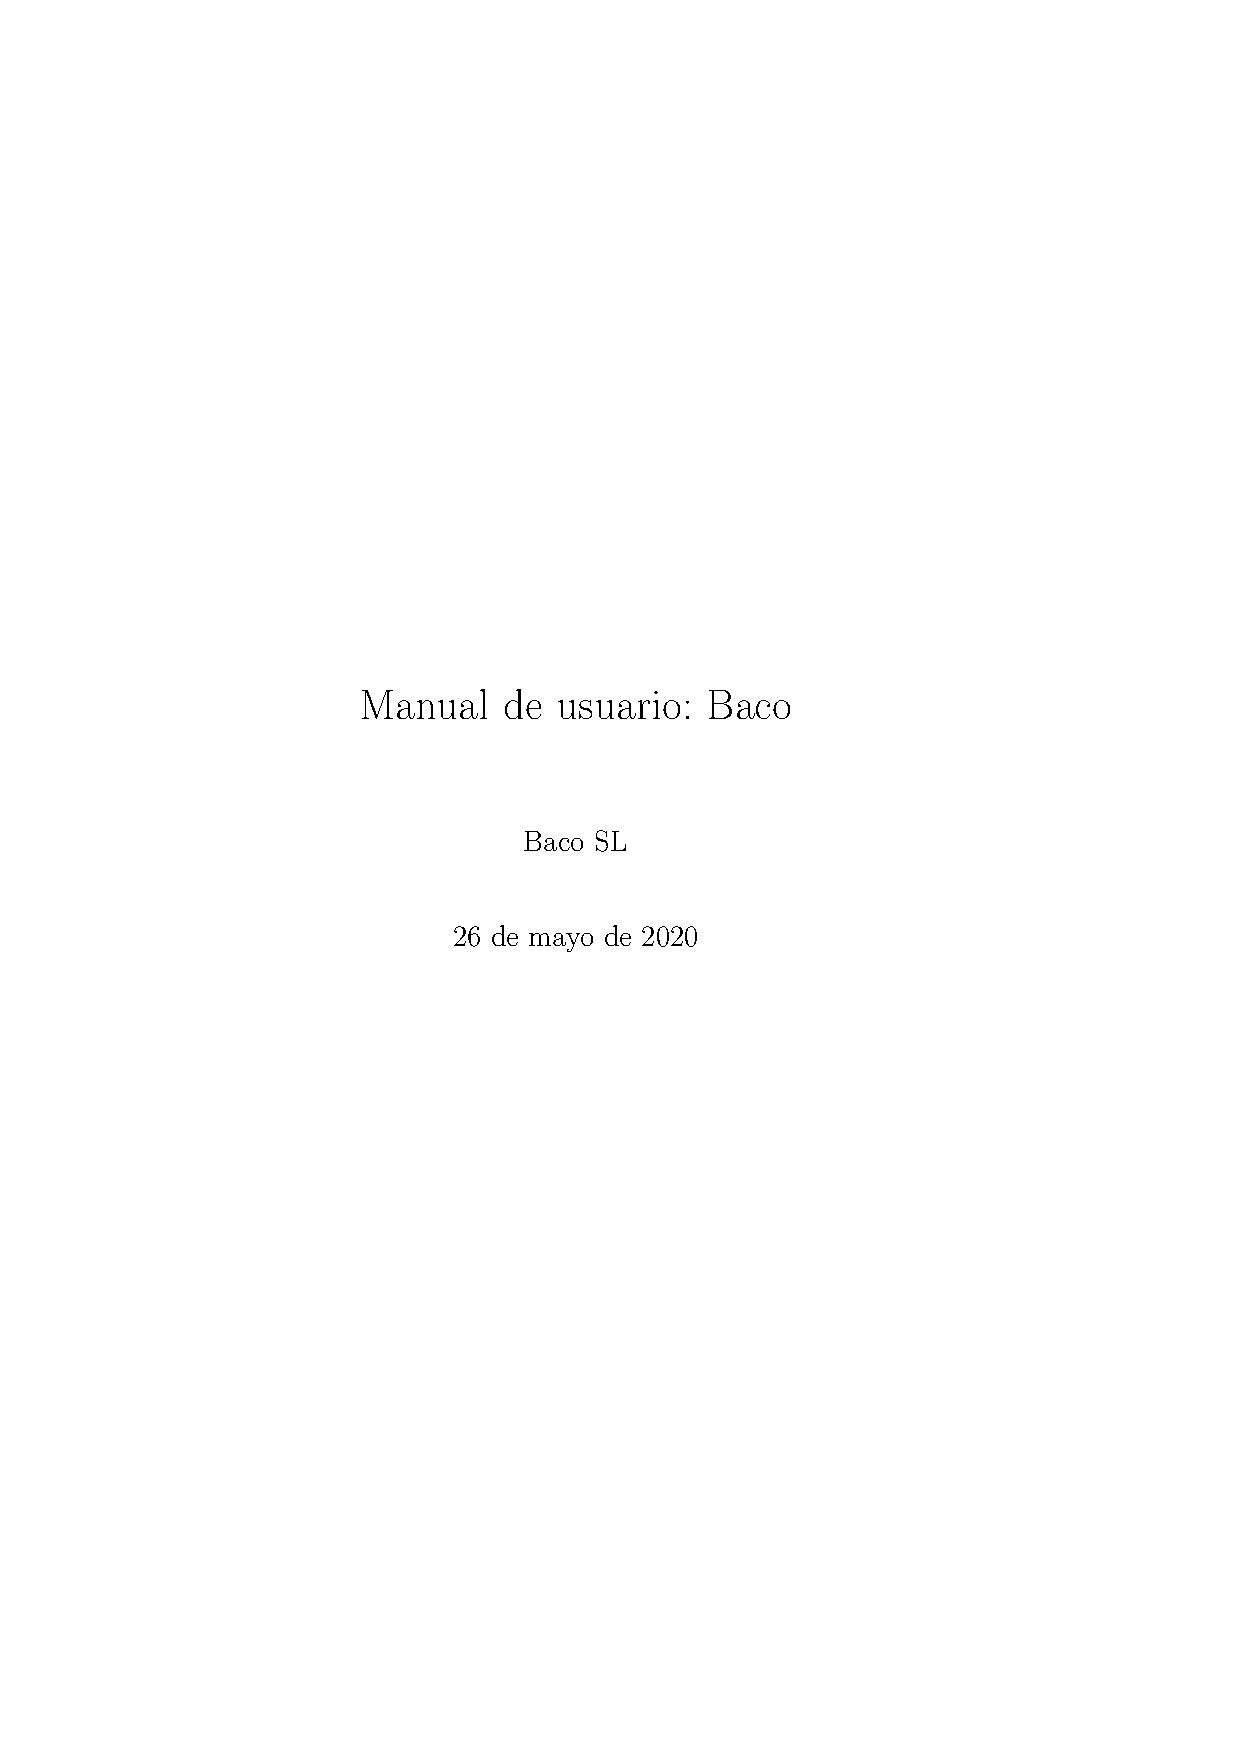
\includepdf[pages=-, frame, scale=.75, pagecommand={}]{../ClientManual/manual.pdf}
		\cleardoublepage
		\section{BacoServer}
		Anexado en esta sección se encuentra el manual de usuario de BacoServer. Véase que la sintaxis empleada en él no es la misma que en el manual de usuario de Baco, sino más técnica.
		\cleardoublepage
		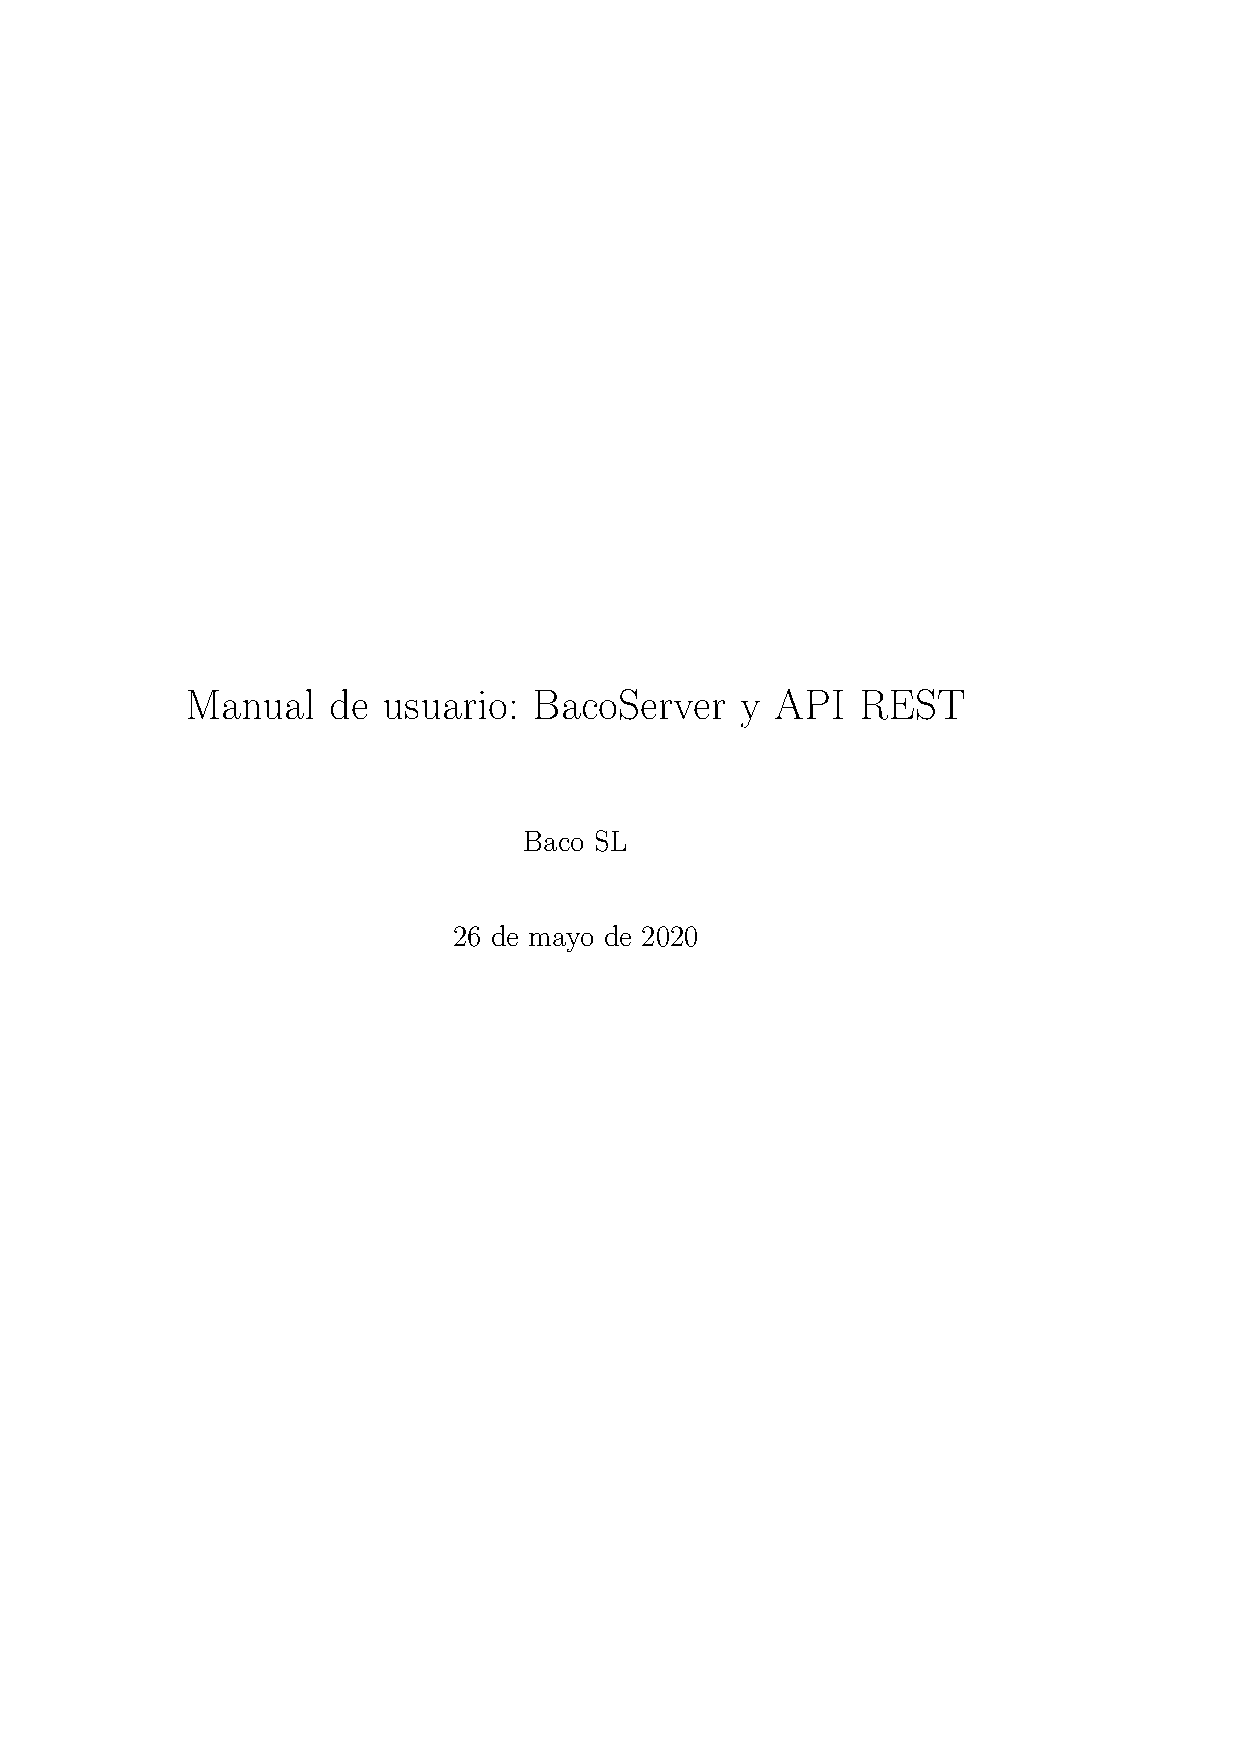
\includepdf[pages=-, frame, scale=.75, pagecommand={}]{../ServerManual/manual.pdf}
		\cleardoublepage
	\chapter{Ficheros entregados} \label{ch:files}
	En los ficheros que se hace entrega se encuentra:
	\begin{itemize}
		\item Una solución de Visual Studio con todos los fuentes necesarios para compilar la API, el cliente y el servidor.
		\item Las instrucciones necesarias en T-SQL para la creación de las tablas en SSMS (incluidas en la \crthypercref{sbc:db}).
		\item Un instalador (wizard) de la aplicación y del servidor.
		\item \hypertarget{netcoredll}{Un fichero comprimido con los ficheros necesarios para la ejecución del API REST. Dado que es una aplicación .NET Core 3.1 el instalador daría como resultado una biblioteca de clases; esto es debido a que puede ser ejecutado desde cualquier plataforma, no solo Windows. Por ello se han incluido los resultados de la compilación en el fichero comprimido en ZIP (dentro de la carpeta de los instaladores).}
		\item Manuales de usuario (incluido en el \crthypercref{ch:man}).
		\item Memoria del trabajo (este documento).
	\end{itemize}
	\chapter{Instalación y requisitos}
		\section{Instalación}
		En esencia, los proyectos entregados son tres: el cliente, el servidor y el API REST. En os tres siguiente puntos se explicará como se instalan o ejecutan. Los instaladores son los de la aplicación de cliente (\crthypercref{sbc:clientinstaller}) y el servidor (\crthypercref{sbc:serverinstaller}), y el ejecutable viene en la \crthypercref{sbc:apirestexe} por los motivos explicados en el \hyperlink{netcoredll}{punto cuatro} del \crthypercref{ch:files}. Los instaladores, por defecto, crearán accesos directos en el escritorio del usuario.
			\subsection{Intalación de Baco} \label{sbc:clientinstaller}
			La ruta por defecto seá en archivos de programa y en la carpeta Baco SL. Dentro se generará una carpeta con el nombre de Baco y en su interior se encontrarán todos los ficheros necesarios para el funcionamiento de la aplicación del cliente.
			\subsection{Intalación del servidor de Baco} \label{sbc:serverinstaller}
			El servidor posee el mismo instalador que la aplicación del cliente y se instala en la misma localización, con la diferencia de que la carpeta que se crea se llamará BacoServer. En su interior podremos apreciar que se incluye la aplicación de cliente. Esto es debido a que para que el servidor funcione requiere de características del cliente, pero el cliente no requiere de características del servidor. En cierta manera, instalando el servidor se instala en cliente. También apréciese que lo usual no será que el usuario instale el servidor en su ordenador, si cabe quizá una empresa pueda requerir de un servidor privado.
			\subsection{Árbol de directorios de la carpeta <<Baco SL>>}
			Dentro de la carpeta donde, por defecto, se alojan los programas, encontramos la siguiente estructura de carpetas:
			\dirtree{%
				.1 Baco SL.
				.2 Baco.
				.3 ....
				.3 Baco.exe.
				.2 BacoServer.
				.3 ....
				.3 Baco.exe.
				.3 BacoServer.exe.
			}
			Donde los ficheros *.exe son los que podremos encontrar como accesos directos en el escritorio.
			\subsection{Puesta en marcha del API REST} \label{sbc:apirestexe}
			Se ha entregado un fichero comprimido dentro de la carpeta de instaladores que contiene los ficheros fuente del API REST. Si se descomprime se vera una carpeta denominada <<API REST>> y dentro se podrá encontrar el ejecutable del API REST. Dicho ejecutable se denomina <<ApiBaco.exe>>.
		\section{Requisitos}
		Los requisitos no difieren de los de cualquier otra aplicación; a continuación se enumerarán y explicará el por qué de ellos:
		\begin{itemize}
			\item Conexión a Internet: dado que los datos están almacenados en Azure, para que el API REST acceda a ellos debe de tener conexión a Internet.
			\item Tarjeta gráfica de gama baja: no se requiere mucha potencia gráfica, pero para la captura de pantalla y el renderizado de vídeo se requiere de computación gráfica. En los casos de pruebas con una Gigabyte GeForce GTX 550 Ti 1GB GDDR5 los clientes no superaban el 5\% de uso de la GPU al enviar y recibir vídeo a la vez.
			\item 2GB de RAM: si bien es cierto que hoy en día lo normal es encontrar memorias de 4GB para arriba, Baco no requiere de gran uso de memoria, menos de 500MB y suponiendo que el programa está al 100\% de sus funcionalidades.
			\item Procesador de gama baja: dado que mucha de la carga potencial de procesamiento de datos se la lleva la GPU, la CPU no recibe una carga muy grande. Durante las pruebas en un Intel Core i5-3570 de 3.80 GHz no superaba el 10\% de CPU al 100\% de sus funcionalidades.
			\item Espacio disponible de 20MB: puesto que es un programa muy simple requiere de una capacidad muy reducida.
		\end{itemize}
	
	\chapter{Conclusiones}
	Pese al poco tiempo que se han hecho prácticas presenciales, gracias a ello se ha podido realizar el trabajo en SSML con T-SQL e implementarlo en Visual Studio para realizar el API REST en C\#. Durante el tiempo que se estuvo en la empresa se enseñó también un control más amplío de LINQ y que, sin duda, queda plasmado en el proyecto.
		\section{Conclusiones sobre el trabajo realizado}
		Se seguiría ampliando y añadiendo funcionalidades, todo cuanto hay en la aplicación ha hecho que se comprendan a fondo multitud de aspectos de programación: manejo de grandes cantidades hilos, la importancia de un código óptimo, la transmisión de datos por Internet a bajo nivel, importancia y control de eventos, y un largo etcétera.
		\section{Posibles ampliaciones y mejoras}
		La mentalidad de Baco es el mantenimiento por parte de su comunidad y el canal oficial, como bien se expresó en la \crthypercref{sc:objetivo}. De todos modos, se tienen prestaciones pensadas para añadir a la aplicación (orden de prioridad):
		\begin{itemize}
			\item Control de los periféricos (teclado y ratón) de usuarios en llamada.
			\item Confirmación de creación de cuenta con el correo electrónico.
			\item Un apartado de opciones más amplio.
			\item Mejora de envío de mensajes de texto: la adición de Markdown daría lugar a un texto más enriquecido.
			\item Optimización de la recepción de video: el vídeo se envía con una tasa de fotogramas alta, pero queda limitada por la velocidad de renderizado del receptor. Una mejor transmisión de los paquetes de vídeo facilitaría la tasa de fotogramas por segundo.
			\item Transmisión de vídeo grabado por la cámara de web.
			\item Una correcta separación de clases: si se separan las clases que se encargan de modificar los aspectos visuales de la aplicación y se encapsulan en una librería las clases <<cerebro>> (aquellas que realizan las tareas imprescindibles de la aplicación, como el envío y la recepción de datos, el manejo de estos...) se podría, fácilmente, exportar Baco a plataformas móviles (Xamarin) y entornos web (ASP.NET): tan solo habría que diseñar su GUI.
		\end{itemize}
		
	\backmatter
	
	\lstlistoflistings \addcontentsline{toc}{chapter}{Lista de Códigos}
	
	\bibliographystyle{apalike-es}
	\bibliography{bibliografia}
	
	\cleardoublepage \clearpage \pagestyle{empty} \vspace*{\fill}
	
\end{document}